
%%%%%%%%%%%%%%%%%%%%%%%%%%%%%%%%%%%%%%%%%%%%%%%%%%%%%%%%%%%%%%%%%%%%
%%%%%%%%%%%%%JIBLM Formatting Package%%%%%%%%%%%%%%%%%%%%%%%%%%%%%%
%%%%%%%%%%%%%Version 1.2: August, 2008%%%%%%%%%%%%%%%%%%%%%%%%%%%
%%%%%%%%%%%%%Author: Paul J. Kapitza, Berry College%%%%%%%%%%%%%%%%
%%%%%%%%%%%%%%%%%%%%%%%%%%%%%%%%%%%%%%%%%%%%%%%%%%%%%%%%%%%%%%%%%%%

\documentclass[oneside]{book}
%%%%%%%%%%%%%journal additions%%%%%%%%%%%%%%%%%%%%%%%%%%%%%%%%%%%%%
\usepackage{time}%make system time available
\usepackage{enumerate}%extended enumeration package
%%%%%%%%%%%%%Symbol libraries%%%%%%%%%%%%%%%%%%%%%%%%%%%%%%%%%%%%%
\usepackage{amssymb}
\usepackage{amsmath}
\usepackage{latexsym}
\usepackage{amsthm}%extended ams-theorem environment

\usepackage{lettrine}%Drop-caps for Masthead
\usepackage{mathptmx}%Times Roman type package for both math and text


\usepackage{endnotes}%Footnotes to the instructor.
   
   
   
   
%%%%%%%%%%%%%Header Customization%%%%%%%%%%%%%%%%%%%%%%%%%%%%%%%%%
\usepackage{fancyhdr}%Header customization
\pagestyle{fancy}
%%%%%%%%%%%%%Chapter headings%%%%%%%%%%%%%%%%%%%%%%%%%%%%%%%%%
\renewcommand{\chaptermark}[1] {\markboth{#1}{}}%

%%%%%%%%%%%%%Page Formatting%%%%%%%%%%%%%%%%%%%%%%%%%%%%%%%%%%
\setlength{\oddsidemargin}{63pt}%%%%%One-sided printing values for 10pt. text-Remove for two sided print
\setlength{\evensidemargin}{63pt}%%%%%One-sided printing values for 10pt. text-Remove for two sided print

\setlength{\parskip}{1mm}
\setlength{\textwidth}{5.0in}
\setlength{\textheight}{8.0in}

%%%%%%%%%%%%%%%%%%%%%%%%%%%%AUTHOR MASTHEAD%%%%%%%%%%%%%%%%%%%%%%%%%%%%%
\newcommand{\authormasthead}{
\begin{flushleft}
\hspace{8.0mm}
\rule{0.3\linewidth}{0.3mm}
\lettrine[lines=2]{D}{raft \rule[3pt]{10mm}{0.5pt} Draft \rule[3pt]{10mm}{0.5pt} Draft \rule[3pt]{10mm}{0.5pt} Draft}
\rule{0.3\linewidth}{0.3mm}
%\hspace{1mm} Issue~\textbf{#1}, Volume #2        Issue 1 (August, 2007)
\vspace{0.2in}
\end{flushleft}
}
%%%%%%%%%%%%%%%%%%%%%%%%%%%%AUTHOR MASTHEAD%%%%%%%%%%%%%%%%%%%%%%%%%%%%%

%%%%%%%%%%%%%%%%%%%%%%%%%%%%TIMESTAMP%%%%%%%%%%%%%%%%%%%%%%%%%%%%%
%%Uses the ``time" package to stamp the time-Editing Feature
\newcommand{\timestamp}{{Edited: \texttt{\now , \today}}}
%%%%%%%%%%%%%%%%%%%%%%%%%%%%TIMESTAMP%%%%%%%%%%%%%%%%%%%%%%%%%%%%%


\let\affiliation\date


%%%%%%%%%%%%%%%%%%%%%%%%%%%% TITLEPAGE%%%%%%%%%%%%%%%%%%%%%%%%%%%%%
%
\makeatletter
\def\maketitle{%
  \null
  \thispagestyle{empty}%
  \timestamp
  \authormasthead
  %\vfill
  \normalfont
  \vspace{2in}
\begin{center}\leavevmode
{\Huge \@title\par}%
\vspace{20mm}
{\Large \@author\par}%
\vspace{5mm}
{\Large \@date\par}% pass affiliation
{\Large \ }
\end{center}
  \vfill
  \null
  \cleardoublepage
 \let\newauthor\@author%transfer to footer line
 }%
\makeatother
%%%%%%%%%%%%%%%%%%%%%%%%%%%% END OF TITLEPAGE%%%%%%%%%%%%%%%%%%%%%%%%%%%%%

%Customized headers and footers- replace authorname with register
\lhead{ \leftmark} \chead{} \rhead{\thepage}
\lfoot{\newauthor} \cfoot{} \rfoot{\emph{DRAFT -- DRAFT -- DRAFT}}
\renewcommand{\headrulewidth}{0.4pt}
\renewcommand{\footrulewidth}{0.4pt}
%
%%%%%%%%%%%%%%%%%%%%%%%%%%%% Annotation Environment %%%%%%%%%%%%%%%%%%%%%%%%%%%%%
\usepackage{comment}
\newcommand{\InstructorVersion}{\includecomment{annotation}}
\newcommand{\StudentVersion}{\excludecomment{annotation}}
%%%%%%%%%%%%%%%%%%%%%%%%%%%% END OF Annotation Environment%%%%%%%%%%%%%%%%%%%%%%%%%%%%%



%%%%%%%%%%%%%%%%%%%%%%%%%%%% Begin--Sectioning Redefines%%%%%%%%%%%%%%%%%%%%%%%%%%%%%
%
\makeatletter
\renewcommand{\@makechapterhead}[1]{%
\vspace*{50\p@}%
  {\parindent \z@ \raggedright \normalfont
    \ifnum \c@secnumdepth >\m@ne
      \if@mainmatter
        \huge \@chapapp\space \thechapter                
        \par\nobreak
        \vskip 20\p@
      \fi
    \fi
    \interlinepenalty\@M
    \LARGE\bfseries  #1\par\nobreak                        
    \vskip 40\p@
  }}


\renewcommand{\@makeschapterhead}[1]{%
  \vspace*{50\p@}%
  {\parindent \z@ \raggedright
    \normalfont
    \interlinepenalty\@M
    \LARGE\bfseries  #1\par\nobreak                      
    \vskip 40\p@
  }}

\makeatother
%%%%%%%%%%%%%%%%%%%%%%%%%%%% End--Sectioning Redefines%%%%%%%%%%%%%%%%%%%%%%%%%%%%%




%%%%%%%%%%Theorem Environments%%%%%%%%%%%%%%%%%%%%%%%%
\newtheorem{theorem}{Theorem}
\newtheorem{acknowledgment}[theorem]{Acknowledgment}
\newtheorem{algorithm}[theorem]{Algorithm}
\newtheorem{axiom}[theorem]{Axiom}
\newtheorem{case}[theorem]{Case}
\newtheorem{claim}[theorem]{Claim}
\newtheorem{conclusion}[theorem]{Conclusion}
\newtheorem{condition}[theorem]{Condition}
\newtheorem{conjecture}[theorem]{Conjecture}
\newtheorem{corollary}[theorem]{Corollary}
\newtheorem{criterion}[theorem]{Criterion}
\newtheorem{definition}[theorem]{Definition}
\newtheorem{example}[theorem]{Example}
\newtheorem{exercise}[theorem]{Exercise}
\newtheorem{lemma}[theorem]{Lemma}
\newtheorem{notation}[theorem]{Notation}
\newtheorem{problem}[theorem]{Problem}
\newtheorem{proposition}[theorem]{Proposition}
\newtheorem{remark}[theorem]{Remark}
\newtheorem{solution}[theorem]{Solution}
\newtheorem{summary}[theorem]{Summary}
%%%%%%%%%%Theorem Environments%%%%%%%%%%%%%%%%%%%%%%%%
%%%%%%%%%%%%%%%%%%%%%%%%%%%%%%%%%%%%%%%%%%%%%%%%%%%%%%%%%%%%%%%%%%%
%%%%%%%%%%%%%JIBLM Formatting Package%%%%%%%%%%%%%%%%%%%%%%%%%%%%%%
%%%%%%%%%%%%%Version 1.2: August, 2008%%%%%%%%%%%%%%%%%%%%%%%%%%%
%%%%%%%%%%%%%Author: Paul J. Kapitza, Berry College%%%%%%%%%%%%%%%%
%%%%%%%%%%%%%%%%%%%%%%%%%%%%%%%%%%%%%%%%%%%%%%%%%%%%%%%%%%%%%%%%%%%
% Modifications marked with DJH

\RequirePackage{xcolor} %% DJH (Otherwise you get a bunch of warnings)
\documentclass[oneside]{book}
%%%%%%%%%%%%%journal additions%%%%%%%%%%%%%%%%%%%%%%%%%%%%%%%%%%%%%
\usepackage{time}%make system time available
\usepackage{enumerate}%extended enumeration package
%%%%%%%%%%%%%Symbol libraries%%%%%%%%%%%%%%%%%%%%%%%%%%%%%%%%%%%%%
% DJH % \usepackage{amssymb}
\usepackage{amsmath}
\usepackage{latexsym}
\usepackage{amsthm}%extended ams-theorem environment

\usepackage{lettrine}%Drop-caps for Masthead
\usepackage{mathptmx}%Times Roman type package for both math and text


\usepackage{endnotes}%Footnotes to the instructor.

\usepackage[letterpaper, margin=1.0in]{geometry} % DJH: Wider margins
\usepackage[charter]{mathdesign} % DJH: Different font


%%%%%%%%%%%%%Header Customization%%%%%%%%%%%%%%%%%%%%%%%%%%%%%%%%%
\usepackage{fancyhdr}%Header customization
\pagestyle{fancy}
%%%%%%%%%%%%%Chapter headings%%%%%%%%%%%%%%%%%%%%%%%%%%%%%%%%%
\renewcommand{\chaptermark}[1] {\markboth{#1}{}}%

%%%%%%%%%%%%%Page Formatting%%%%%%%%%%%%%%%%%%%%%%%%%%%%%%%%%%
%DJH %\setlength{\oddsidemargin}{63pt}%%%%%One-sided printing values for 10pt. text-Remove for two sided print
%DJH %\setlength{\evensidemargin}{63pt}%%%%%One-sided printing values for 10pt. text-Remove for two sided print

\setlength{\parskip}{1mm}
% DJH % \setlength{\textwidth}{5.0in}
% DJH % \setlength{\textheight}{8.0in}

%%%%%%%%%%%%%%%%%%%%%%%%%%%%AUTHOR MASTHEAD%%%%%%%%%%%%%%%%%%%%%%%%%%%%%
\newcommand{\authormasthead}{
\begin{flushleft}
\hspace{8.0mm}
\rule{0.3\linewidth}{0.3mm}
\lettrine[lines=2]{D}{raft \rule[3pt]{10mm}{0.5pt} Draft \rule[3pt]{10mm}{0.5pt} Draft \rule[3pt]{10mm}{0.5pt} Draft}
\rule{0.3\linewidth}{0.3mm}
%\hspace{1mm} Issue~\textbf{#1}, Volume #2        Issue 1 (August, 2007)
\vspace{0.2in}
\end{flushleft}
}
%%%%%%%%%%%%%%%%%%%%%%%%%%%%AUTHOR MASTHEAD%%%%%%%%%%%%%%%%%%%%%%%%%%%%%

%%%%%%%%%%%%%%%%%%%%%%%%%%%%TIMESTAMP%%%%%%%%%%%%%%%%%%%%%%%%%%%%%
%%Uses the ``time" package to stamp the time-Editing Feature
\newcommand{\timestamp}{{Edited: \texttt{\now , \today}}}
%%%%%%%%%%%%%%%%%%%%%%%%%%%%TIMESTAMP%%%%%%%%%%%%%%%%%%%%%%%%%%%%%


\let\affiliation\date


%%%%%%%%%%%%%%%%%%%%%%%%%%%% TITLEPAGE%%%%%%%%%%%%%%%%%%%%%%%%%%%%%
%
\makeatletter
\def\maketitle{%
  \null
  \thispagestyle{empty}%
  \timestamp
  \authormasthead
  %\vfill
  \normalfont
  \vspace{2in}
\begin{center}\leavevmode
{\Huge \@title\par}%
\vspace{20mm}
{\Large \@author\par}%
\vspace{5mm}
{\Large \@date\par}% pass affiliation
{\Large \ }
\end{center}
  \vfill
  \null
  \cleardoublepage
 \let\newauthor\@author%transfer to footer line
 }%
\makeatother
%%%%%%%%%%%%%%%%%%%%%%%%%%%% END OF TITLEPAGE%%%%%%%%%%%%%%%%%%%%%%%%%%%%%

%Customized headers and footers- replace authorname with register
\lhead{ \leftmark} \chead{} \rhead{\thepage}
\lfoot{Hunter $<$ Morrow} \cfoot{} \rfoot{\emph{DRAFT -- DRAFT -- DRAFT}} %DJH
\renewcommand{\headrulewidth}{0.4pt}
\renewcommand{\footrulewidth}{0.4pt}
%
%%%%%%%%%%%%%%%%%%%%%%%%%%%% Annotation Environment %%%%%%%%%%%%%%%%%%%%%%%%%%%%%
\usepackage{comment}
\newcommand{\InstructorVersion}{\includecomment{annotation}}
\newcommand{\StudentVersion}{\excludecomment{annotation}}
%%%%%%%%%%%%%%%%%%%%%%%%%%%% END OF Annotation Environment%%%%%%%%%%%%%%%%%%%%%%%%%%%%%



%%%%%%%%%%%%%%%%%%%%%%%%%%%% Begin--Sectioning Redefines%%%%%%%%%%%%%%%%%%%%%%%%%%%%%
%
\makeatletter
\renewcommand{\@makechapterhead}[1]{%
\vspace*{50\p@}%
  {\parindent \z@ \raggedright \normalfont
    \ifnum \c@secnumdepth >\m@ne
      \if@mainmatter
        \huge \@chapapp\space \thechapter
        \par\nobreak
        \vskip 20\p@
      \fi
    \fi
    \interlinepenalty\@M
    \LARGE\bfseries  #1\par\nobreak
    \vskip 40\p@
  }}


\renewcommand{\@makeschapterhead}[1]{%
  \vspace*{50\p@}%
  {\parindent \z@ \raggedright
    \normalfont
    \interlinepenalty\@M
    \LARGE\bfseries  #1\par\nobreak
    \vskip 40\p@
  }}

\makeatother
%%%%%%%%%%%%%%%%%%%%%%%%%%%% End--Sectioning Redefines%%%%%%%%%%%%%%%%%%%%%%%%%%%%%




%%%%%%%%%%%Theorem Environments%%%%%%%%%%%%%%%%%%%%%%%%
%% \newtheorem{theorem}{Theorem}[chapter] % DJH
%\theoremstyle{definition} % DJH
%\newtheorem{acknowledgment}[theorem]{Acknowledgment}
%\newtheorem{algorithm}[theorem]{Algorithm}
%\newtheorem{axiom}[theorem]{Axiom}
%\newtheorem{case}[theorem]{Case}
%\newtheorem{claim}[theorem]{Claim}
%\newtheorem{conclusion}[theorem]{Conclusion}
%\newtheorem{condition}[theorem]{Condition}
%\newtheorem{conjecture}[theorem]{Conjecture}
%\newtheorem{corollary}[theorem]{Corollary}
%\newtheorem{criterion}[theorem]{Criterion}
%\newtheorem{definition}[theorem]{Definition}
%\newtheorem{example}[theorem]{Example}
%\newtheorem{exercise}[theorem]{Exercise}
%\newtheorem{lemma}[theorem]{Lemma}
%\newtheorem{notation}[theorem]{Notation}
%\newtheorem{proposition}[theorem]{Proposition}
%\newtheorem{remark}[theorem]{Remark}
%\newtheorem{solution}[theorem]{Solution}
%\newtheorem{summary}[theorem]{Summary}
%% \newtheorem{problem}{Problem} %DJH
%%%%%%%%%%Theorem Environments%%%%%%%%%%%%%%%%%%%%%%%%
 % My customized version
\usepackage{graphicx}
\usepackage{enumitem}
%%%% enumitem declarations
\newlist{problemparts}{enumerate}{1}
\setlist[problemparts,1]{label=(\alph*), itemsep=0pt, topsep=3pt}

\usepackage{thmtools}
%%%% thmtools declarations
\theoremstyle{definition}
\declaretheorem[numberwithin=chapter]{definition}
\declaretheorem[shaded={bgcolor=white}]{problem}
\declaretheorem[sibling=definition]{theorem}
\declaretheorem[sibling=definition]{lemma}
\declaretheorem[sibling=definition]{axiom}

\usepackage{amscd} % For commutative diagrams
\usepackage{tikz} % For field diagrams
\usetikzlibrary{shapes.misc}


%%%% Customize endnote format
%\newcommand*\notesymbol[1]{\tikz[baseline=(char.base)]{
%           \node[shape=rectangle,fill=yellow!20,draw,inner sep=2pt] (char) {#1};}}
\newcommand*\notesymbol[1]{\tikz{
            \node[shape=rounded rectangle,fill=yellow!25,draw,inner xsep=2pt, inner ysep=2pt] (char) {#1};}}
\renewcommand{\makeenmark}{\notesymbol{\scriptsize\theenmark}\hspace{3pt}}

%%%% Useful abbreviations
\newcommand{\ZZ}{\mathbb{Z}}
\newcommand{\NN}{\mathbb{N}}
\newcommand{\QQ}{\mathbb{Q}}
\newcommand{\RR}{\mathbb{R}}
\newcommand{\CC}{\mathbb{C}}
\newcommand{\FF}{\mathbb{F}}
\DeclareMathOperator{\stab}{stab}
\DeclareMathOperator{\Irr}{Irr}
\DeclareMathOperator{\Gal}{Gal}
\DeclareMathOperator{\Ker}{Ker}

%
%%%%%%%%%%%%%%%%%%%%% Annotation Environment Switch%%%%%%%%%%%%
%\StudentVersion
\InstructorVersion
%%%%%%%%%%%%%%%%%%%%% Annotation Environment Switch%%%%%%%%%%%%
%
\newcommand\blfootnote[1]{%
  \begingroup
  \renewcommand\thefootnote{}\footnote{#1}%
  \addtocounter{footnote}{-1}%
  \endgroup
}

\begin{document}
\large
\frontmatter
\title{Abstract Algebra I \& II}
\author{David J. Hunter$^1$ $<$ Margaret L. Morrow$^{2\dagger}$}
\affiliation{$^1$Westmont College \\ $^2$SUNY Plattsburgh}
\blfootnote{$^\dagger$The relation ``Hunter $<$ Morrow'' indicates that Chapters 1--5 of these notes were originally written by Margaret Morrow. David Hunter revised these chapters and added Chapters 6--13, and he takes full responsibility for this version of these notes.}
\maketitle

\tableofcontents

%%%%%%%%%%%%%%%%%%%%%%%%%%%%%%%%%%%%To the Instructor%%%%%%%%%%%%%%%%%%%%%%%%%%%%%%%%

\begin{annotation}
 \chapter{To the Instructor}

These notes provide an introduction to abstract algebra for advanced undergraduate mathematics majors. There should be enough material for a two-semester sequence. At Westmont College, most mathematics majors and some minors take first semester of this sequence, which (ambitiously) covers Chapters 1--9. These chapters contain a fairly standard treatment of groups, rings, and fields. Some of the more motivated mathematics majors, especially those destined for graduate school, will continue to the second semester, completing Chapters 10--13. The second semester includes some advanced group theory, including Sylow Theory, but its ultimate goal is to introduce students to Galois Theory.

This ultimate goal guides the selection of topics throughout these notes, beginning with the introductory activity. On the first day of class, students will discover how group operations can describe the symmetries of a polygon as permutations of the vertices. Analogously, by the end of the second semester, students will be using groups to describe automorphisms of splitting fields as permutations of the roots of a polynomial. It helps to keep the goal of the Galois correspondence in mind throughout both semesters, as it serves as a unifying theme.

At Westmont, enrollment for the first semester of this sequence is typically between 10 and 20, and second semester enrollment is much smaller. Regardless of class size, these notes are designed to be used with some form of the Moore method. Depending on the strength of the class, this method can be modified to provide additional support and scaffolding for students. I have found it very helpful to include the following components.
\begin{itemize}
    \item \textbf{Prework.} Before class, students should work independently on a selection of problems. I like to collect these preliminary solutions, either via online submissions or by running them through a scanner at the beginning of class. I grade these very leniently, giving full credit for what appears to be honest engagement with the problems. Currently, solutions to nearly every problem in every abstract algebra text can be found by searching the Internet, so lenient grading at this stage is essential. I tell students not to use any outside resources during the Prework stage, because I would rather see a half-right attempt at a problem of their own construction than a regurgitation of somebody else's solution.
    \item \textbf{Class Discussion.} During class, students will benefit by explaining their solutions, or lack thereof, to each other. These conversations can be encouraged in a variety of ways, using small-group discussion, class presentations, or a combination of the two. The goal of these discussions is to come to some consensus about a correct solution to each problem.
    \item \textbf{Postwork.} After class, students should be able to write up complete and correct solutions to every problem. These write-ups can be posted on a class wiki, maintained in a code repository, collected through a course management system, or kept in a journal. I carefully grade some subset of these assignments, where the subset size is determined by the size of the class.
\end{itemize}

Due to the abstract nature of the subject, it is important for instructors to provide some sort of regular framing and perspective on the material. Lectures will typically not be necessary, but students will appreciate hearing about why these techniques were developed and how these topics fit together.

As the sequence of problems progresses, the difficulty level tends to increase. Early on, students should be able to grapple with every detail of every proof. In later material, especially in the development of the Galois correspondence, some of the more difficult theoretical hurdles are given as theorems, with outlines, or ``sketches,'' of proofs. Often undergraduate treatments of Sylow and Galois theory simply state the main theorems and have students do calculations. While these notes do not require students to construct proofs of every theorem, they are designed to expose students to the theoretical development of the important results.

Throughout the Instructor Version of these notes, you will notice numbers $m$ typeset as \notesymbol{\scriptsize $m$} at the end of some of the problems. These numbers refer to endnotes in the last Chapter titled, ``Notes to the Instructor.'' These endnotes, which are hidden in the Student Version, provide advice about additional exposition that should be provided by the instructor.

\section*{Acknowledgements}

Chapters 1--5 were originally written by Margaret Morrow and published on \texttt{jiblm.org}. I have made some modifications to these chapters, but they retain much of her original content. I have added Chapters 6--13, the contents of which is heavily influenced by some of my favorite algebra texts, including the following.
\begin{itemize}
    \item \textit{A First Course in Abstract Algebra}, by John Fraleigh.
    \item \textit{A First Course in Abstract Algebra}, by Joseph Rotman.
    \item \textit{Contemporary Abstract Algebra}, by Joseph Gallian.
    \item \textit{Algebra}, by Thomas Hungerford.
    \item \textit{Galois Theory}, by Joseph Rotman.
\end{itemize}

References in square brackets in the instructors' notes refer to these sources.

\begin{flushright}
--- David J. Hunter, Westmont College, July 2018
\end{flushright}

\end{annotation}


%%%%%%%%%%%%%%%%%%%%%%%%%%%%%%%%%%%%To the Student%%%%%%%%%%%%%%%%%%%%%%%%%%%%%%%%

\chapter{To the Student}

Have you ever wondered how modern mathematics came to be? To what extent are the definitions and theorems that we find in the canonical textbooks the result of choices made by historical figures? Is there something intrinsic to the subject that forces modern mathematical theory down the path that it takes? Put another way, would Earthling mathematicians recognize the work of a community of mathematicians from a distant galaxy?

We can glean some insight into these questions by proceeding axiomatically: make as few assumptions and definitions as possible, and see where logical deduction leads. The material in these notes represents the consequences of some very low-level mathematical foundations: logic, sets, and the integers. These consequences have applications throughout pure and applied mathematics, and are part of the \textit{lingua franca} of the discipline.

Historically, much of this subject was motivated by the search for solutions to polynomial equations.  There is a well-known formula for solving any quadratic polynomial equation, but are there analogs to this formula for polynomials of degree greater than~2? It is easy to believe that our hypothetical space-alien mathematical colleagues would also be interested in such formulas, but mathematical theory required to answer this question turns out to be surprisingly deep.

 Throughout this semester and the next (should you persevere), you will be guided through a series of deductive discoveries along the path that modern mathematicians have blazed. Whether this path is the only reasonable one will be yours to judge once you have completed the journey.

\begin{quote}
  \textit{That student is taught the best who is told the least.} ---R. L. Moore
\end{quote}

These notes (along with the sequel) give a comprehensive coverage of two semesters of advanced undergraduate or beginning graduate algebra. However, these notes contain mostly questions, and you must supply the answers. Your written accounts of your inquiry and our class discussions will produce a complete abstract algebra textbook of your own construction.

\mainmatter

\chapter*{Introductory Activity: Some Useful Examples}
\addcontentsline{toc}{chapter}{Introductory Activity}
\markboth{Introductory Activity}{Introductory Activity}

\textbf{Example I: Symmetries.}
\begin{annotation}
 \endnote{The introductory activity is designed to be done in groups on the first day of class, after a brief explanation of symmetries. Later material will refer to the examples that it introduces, so it is important not to skip it. You may wish to prepare the cut-out triangles and squares in advance. (Tip: provide only one triangle and one square per group, to encourage collaboration.) This activity also gives students a chance to solve some relatively concrete problems in a relaxed atmosphere. Ideally, each group should be able to send a representative to the board to record their answers. In addition to presenting these useful examples, the goal is to get students accustomed to sharing their work with the rest of the class. If time permits at the end of the group work, an informal whole-class discussion could look for patterns in the multiplication tables.}
\end{annotation}

We can think of a \textit{symmetry} of a plane figure as a rigid motion of the figure that results in the figure simply being repositioned on top of its original outline.

\textit{It is the final position of the figure that is important,} not the motion as such. For example, if we rotate the triangle below through $120^\circ$ or $480^\circ$, the triangle ends up in the same final position, so we do not think of these as distinct symmetries.

\begin{enumerate}
    \item Consider the symmetries of an equilateral triangle, as illustrated below. Each sketch shows the resulting position when the specified motion is applied to the triangle starting in the original position.
\begin{center}
    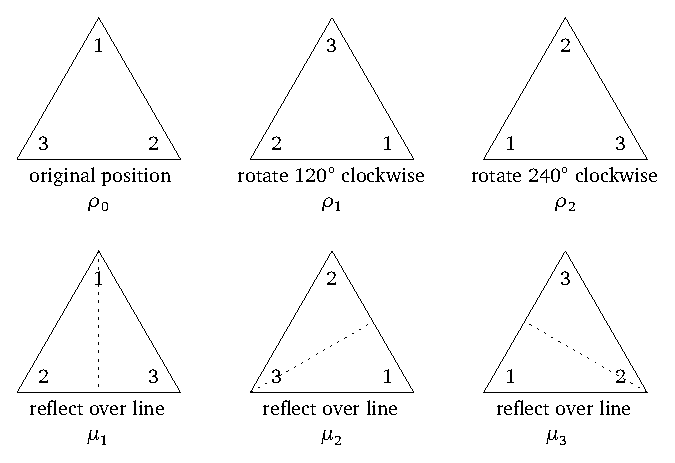
\includegraphics{wstriangles.eps}
\end{center}
    Cut an equilateral triangle out of a sheet of paper, and number the vertices 1, 2, and 3 as shown in the original position. Put the number of each vertex on the back of the triangle as well.

    We can apply one of the rigid motions, and then, \textit{continuing from the new position of the triangle,} apply another of the rigid motions. We can then record the overall effect as one of six symmetries listed above.

    For example if we first apply $\mu_1$, then (continuing from the resulting position) apply $\rho_1$ (a $120^\circ$ clockwise rotation) we end up with $\mu_2$. Using our usual function composition notation, we can write $\rho_1 \circ \mu_1 = \mu_2$.

    It is useful to write the results of all such combinations in table form, as shown below. We show the result of $\rho_1 \circ \mu_1$ in the row labeled $\rho_1$ and the column labeled $\mu_1$.

    \textbf{Important:} The convention is that we enter the result of $\rho_1 \circ \mu_1$ into the row corresponding to $\rho_1$ and the column corresponding to $\mu_1$, even though when we do these motions we first do the reflection $\mu_1$ and then the rotation $\rho_1$.

    \begin{center}
  \renewcommand{\arraystretch}{1.7}
    \begin{tabular}{|c||c|c|c|c|c|c|} \hline
        $\circ$ & $\rho_0$ & $\rho_1$ & $\rho_2$ & $\mu_1$ & $\mu_2$ & $\mu_3$ \\ \hline \hline
        $\rho_0$ & & & & & & \\ \hline
        $\rho_1$ & & & & & & \\ \hline
        $\rho_2$ & & & & & & \\ \hline
        $\mu_1$ & & & & & & \\ \hline
        $\mu_2$ & & & & & & \\ \hline
        $\mu_3$ & & & & & & \\ \hline
    \end{tabular}
    \end{center}

    Use the cut-out triangle to determine the result of all the compositions and complete the table. We will denote this collection of symmetries, together with composition, by $D_3$.

    \item You may have noticed that you can determine which symmetry was performed by looking at the labels of each vertex. Instead of representing rotations and reflections using Greek letters, it is often convenient to represent them using \textit{cycle notation.} For example, starting with the original position, the rotation $\rho_1$ moves vertex 1 to vertex 2, vertex 2 to vertex 3, and vertex 3 to vertex 1.
    \begin{center}
        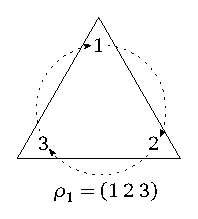
\includegraphics{d3cycles.eps}
    \end{center}
We can denote this rotation with the cycle $(1\; 2\; 3)$, which we read as ``1 goes to 2, 2 goes to 3, 3 goes to 1''. In cycle notation, each vertex moves to the one after it, and the last one wraps around to the first.

Complete the table below, giving the cycle that corresponds to each symmetry.
    \begin{center}
   \renewcommand{\arraystretch}{1.7}
    \begin{tabular}{|c|c|c|c|c|c|} \hline
         $\rho_0$ & $\rho_1$ & $\rho_2$ & $\mu_1$ & $\mu_2$ & $\mu_3$ \\ \hline
         $(1)$ & $(1\; 2\; 3)$ & $\phantom{(1\; 2\; 3)}$ & $(2\; 3)$ & $\phantom{(1\; 2\; 3)}$ & $\phantom{(1\; 2\; 3)}$ \\ \hline
    \end{tabular}
    \end{center}

\clearpage

    \item Develop similar tables for the symmetries of a square. We will use the notation $D_4$ for the symmetries of a square together with composition. Use the symbols indicated in the diagram below to denote the eight symmetries.
    \begin{center}
        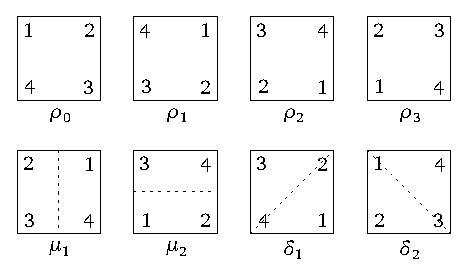
\includegraphics{wssquares.eps}
    \end{center}

    Using a cut-out square (or any other method), compute the compositions and fill out the following table.

    \begin{center}
  \renewcommand{\arraystretch}{1.7}
    \begin{tabular}{|c||c|c|c|c|c|c|c|c|} \hline
        $\circ$ & $\rho_0$ & $\rho_1$ & $\rho_2$ & $\rho_3$ & $\mu_1$ & $\mu_2$ & $\delta_1$ & $\delta_2$ \\ \hline \hline
        $\rho_0$ & & & & & & & &   \\ \hline
        $\rho_1$ & & & & & & & &  \\ \hline
        $\rho_2$ & & & & & & & &  \\ \hline
        $\rho_3$ & & & & & & & &  \\ \hline
        $\mu_1$ & & & & & &  & & \\ \hline
        $\mu_2$ & & & & & &  & & \\ \hline
        $\delta_1$ & & & & & &  & & \\ \hline
        $\delta_2$ & & & & & &  & & \\ \hline
    \end{tabular}
    \end{center}
    In addition, write each symmetry in cycle notation. (Notice that $\rho_2$, $\mu_1$, and $\mu_2$ need to be written as products of two disjoint cycles.)
    \begin{center}
   \renewcommand{\arraystretch}{1.7}
    \begin{tabular}{|c|c|c|c|c|c|c|c|} \hline
         $\rho_0$ & $\rho_1$ & $\rho_2$ & $\rho_3$ & $\mu_1$ & $\mu_2$ & $\delta_1$ & $\delta_2$ \\ \hline
         $(1)$ & $(1\; 2\; 3 \; 4)$ & $\phantom{(1\; 2\; 3\; 4)}$
         & $\phantom{(1\; 2\; 3\; 4)}$
         & $(1\; 2)( 3\; 4)$ & $\phantom{(1\; 2\; 3\; 4)}$ & $\phantom{(1\; 2\; 3\; 4)}$
         & $\phantom{(1\; 2\; 3\; 4)}$ \\ \hline
    \end{tabular}
    \end{center}
\end{enumerate}

\clearpage

\textbf{Example II: Clock arithmetic.} Consider the numbers on a clock, and imagine 0 in place of 12. (We will denote this set by $\mathbb{Z}_{12}$). So $\mathbb{Z}_{12} = \{0,1,2,3,4,5,6,7,8,9,10,11\}$.

We define ``addition modulo 12'' on this set as follows: for $a$ and $b$ in this set, $a + b \pmod{12}$ is the hour on the clock-face that is $b$ hours after $a$. For example, $9 + 5 = 2 \pmod{12}$, since 0 is 3 hours after 9, and we need an additional 2 hours after that.)

We can also define ``multiplication mod 12'' on $\mathbb{Z}_{12}$ by thinking of multiplication as repeated addition modulo 12. So for $a$ and $b$ in $\mathbb{Z}_{12}$, we think of $a\cdot b \pmod{12}$ as the result of adding $b$ to itself $a$ times, modulo 12. For example $3 \cdot 7 = 9 \pmod{12}$.

There is nothing special about 12 here; we can just as easily define addition and multiplication mod $n$ on the set $\{0,1,2,...,n-1\}$ for any fixed positive integer $n$. Simply imagine a clock-face with the numbers $\{0,1,2,...,n-1\}$ in place of $\{0,1,2,3,4,5,6,7,8,9,10,11\}$, and for $a$ and $b$ in this set, define $a+b \pmod{2}$ to be the hour on this clock-face that is $b$ hours after~$a$. Define $a\cdot b \pmod{n}$ to be the result of adding $b$ to itself $a$ times, modulo $n$.

We can draw up tables for these operations, just as we did for symmetries.
\begin{enumerate}
    \item Consider $\mathbb{Z}_5 = \{0,1,2,3,4\}$ Draw up a table for addition mod 5, and a separate table for multiplication mod 5.
    \begin{center}
  \renewcommand{\arraystretch}{1.7}
    \begin{tabular}{|c||c|c|c|c|c|} \hline
        $+$ & $0$ & $1$ & $2$ & $3$ & $4$  \\ \hline \hline
        $0$ & $\phantom{00}$ & $\phantom{00}$ & $\phantom{00}$ & $\phantom{00}$ & $\phantom{00}$ \\ \hline
        $1$ & & & & &  \\ \hline
        $2$ & & & & &  \\ \hline
        $3$ & & & & &  \\ \hline
        $4$ & & & & &  \\ \hline
    \end{tabular}
    \hspace{0.5in}
    \begin{tabular}{|c||c|c|c|c|c|c|} \hline
        $\cdot$ & $0$ & $1$ & $2$ & $3$ & $4$  \\ \hline \hline
        $0$ & $\phantom{00}$ & $\phantom{00}$ & $\phantom{00}$ & $\phantom{00}$ & $\phantom{00}$ \\ \hline
        $1$ & & & & &  \\ \hline
        $2$ & & & & &  \\ \hline
        $3$ & & & & &  \\ \hline
        $4$ & & & & &  \\ \hline
    \end{tabular}
    \end{center}
    \item Consider $\mathbb{Z}_6 = \{0,1,2,3,4,5\}$ Draw up a table for addition mod 6, and a separate table for multiplication mod 6.
    \begin{center}
  \renewcommand{\arraystretch}{1.7}
    \begin{tabular}{|c||c|c|c|c|c|c|} \hline
        $+$ & $0$ & $1$ & $2$ & $3$ & $4$ & $5$ \\ \hline \hline
        $0$ & $\phantom{00}$ & $\phantom{00}$ & $\phantom{00}$ & $\phantom{00}$ & $\phantom{00}$ & $\phantom{00}$ \\ \hline
        $1$ & & & & & & \\ \hline
        $2$ & & & & & & \\ \hline
        $3$ & & & & & & \\ \hline
        $4$ & & & & & & \\ \hline
        $5$ & & & & & & \\ \hline
    \end{tabular}
    \hspace{0.5in}
    \begin{tabular}{|c||c|c|c|c|c|c|} \hline
        $\cdot$ & $0$ & $1$ & $2$ & $3$ & $4$ & $5$ \\ \hline \hline
        $0$ & $\phantom{00}$ & $\phantom{00}$ & $\phantom{00}$ & $\phantom{00}$ & $\phantom{00}$ & $\phantom{00}$ \\ \hline
        $1$ & & & & & & \\ \hline
        $2$ & & & & & & \\ \hline
        $3$ & & & & & & \\ \hline
        $4$ & & & & & & \\ \hline
        $5$ & & & & & & \\ \hline
    \end{tabular}
    \end{center}
\end{enumerate}

\chapter{Introduction to Groups}

In this course, we stipulate the meanings of the terms and symbols using \textit{definitions}. When faced with a new definition, try to understand it by thinking of examples that satisfy the conditions of the definition.  It also helps to try to come up with ``non-examples,'' meaning entities closely related to the defined concept, but that do not conform precisely to the definition.

\begin{definition}
    A \textbf{binary operation} \(*\) on a set \(A\) is a function \(A \times A \rightarrow A\), where \((a,b) \mapsto a*b\).  In other words, a binary operation inputs two elements \(a\), \(b\) of the set \(A\), and outputs a well-defined element \(a * b\) of the set \(A\).
\end{definition}

\begin{problem}\label{prob:binops}
Which of the following are binary operations on the specified set? If not, explain why not.
\begin{problemparts}
  \item Addition on \(\mathbb{Z}\), the set of integers.
  \item Subtraction on \(\mathbb{Z}\), the set of integers.
  \item Subtraction on \(\mathbb{N}\), the set \(\{1,2,3,\ldots\}\) of natural numbers.
  \item Division on \(\mathbb{R}\), the set of real numbers.
  \item Division on \(\mathbb{Z}\setminus \{0\}\).
  \item Composition on \(D_4\), the symmetries of the square.
  \item Composition on the set of rotations in \(D_4\).
  \item Multiplication modulo 6 on \(\mathbb{Z}_6\).
\end{problemparts}
\end{problem}

\begin{definition}
A binary operation is \textbf{associative} if \((a * b)*c = a*(b*c)\) for all \(a,b,c \in A\).  An element \(e\) is said to be an \textbf{identity} for~\(*\) if \(a*e = e*a = a\) for all \(a \in A\).
An element \(b\) is an \textbf{inverse} of the element \(a\) if \(a * b = b * a = e\).
\end{definition}

\begin{problem}
Refer back to those operations in Problem~\ref{prob:binops} that were binary operations.
Do the following for each of these binary operations.
\begin{problemparts}
  \item Determine whether the operation is associative, and if not, prove that the operation is not associative.
  \item State whether there is an identity for the operation, and if so, identify it.
  \item If there is an identity for the operation, determine which elements (if any) have inverses.
\end{problemparts}
\end{problem}

\clearpage % so the definition and problem are together

\begin{definition}
    A binary operation is \textbf{commutative} if \(a * b = b * a\) for all \(a,b \in A\).
\end{definition}

\begin{problem}
Determine which of the binary operations in Problem~\ref{prob:binops} are commutative, and if not, provide proof that the operation is not commutative.
\end{problem}

\begin{problem}
Prove that if a binary operation \(*\) on a set \(A\) has an identity element, then that identity element is unique.
\end{problem}

\begin{definition}
A \textbf{group} is a set \(G\) together with a binary operation \(*\) on \(G\) satisfying the following:
\begin{enumerate}[itemsep=0pt, topsep=3pt]
  \item The operation \(*\) is associative.
  \item There is an element in \(G\) which is an identity for \(*\).
  \item Every element in \(G\) has an inverse with respect to \(*\) in \(G\).
\end{enumerate}
We denote the group by \(\langle G, * \rangle\). We refer to the set \(G\) as the \textbf{underlying set} of the group \(\langle G, * \rangle\). (However if the specific operation is clear from the context, or is not important in the context, we sometimes simply write \(G\) instead of \(\langle G, * \rangle\) for the group, and speak of ``the group \(G\).'')
\end{definition}

\begin{problem}\label{prob:groupex}
Which of the following are groups? If not, explain why not.
\begin{problemparts}
  \item  \(\langle \mathbb{Z}, + \rangle\)
  \item  \(\langle \mathbb{Z}, - \rangle\)
  \item  \(\langle \mathbb{Z}, \times \rangle\)
  \item  \(\langle \mathbb{Z}, \div \rangle\)
  \item  \(\langle \mathbb{R}^+, \times \rangle\) (\(\mathbb{R}^+\) denotes the set of positive real numbers.)
  \item  The set of symmetries of a regular pentagon with operation composition.
  \item  \(\mathbb{Z}_6\) with operation addition mod 6.
  \item  \(\mathbb{Z}_6\) with operation multiplication mod 6.
  \item  \(\mathbb{Z}_6 \setminus \{0\}\) with operation multiplication mod 6.
  \item  \(\mathbb{Z}_5 \setminus \{0\}\) with operation multiplication mod 5.
\end{problemparts}
\end{problem}

\begin{problem}
Prove that the following is, or is not a group, as appropriate.
The set \( S = \mathbb{R} \setminus \{1\} \) with operation defined by \( a * b = a + b - ab \) for all \(a\) and \(b\) in \(S\). (On the right side of the equation, the operations are the usual addition and multiplication in \(\mathbb{R} \).)
\end{problem}

\begin{problem}
Prove that the following is, or is not a group, as appropriate: The set \(M_2(\mathbb{R})\) of all 2 by 2 matrices, with real numbers as entries, and operation matrix multiplication.
\end{problem}

\begin{definition}\label{def:orderofgroup} \mbox{}
\begin{itemize}[itemsep=0pt, topsep=3pt]
  \item A group \( \langle G, * \rangle \) is said to be \textbf{abelian} if \(*\) is commutative.
  \item We say a group is \textbf{finite} if the underlying set contains finitely many elements. We say a group is \textbf{infinite} if the underlying set contains infinitely many elements.
  \item For a finite group \(G\), the \textbf{order} of \(G\) is the number of elements in \(G\). We also say that an infinite group has \textbf{infinite order}.
\end{itemize}
\end{definition}

\begin{problem}
Provide at least two examples of abelian groups.
\end{problem}

\begin{problem}
Refer back to Problem~\ref{prob:groupex}. Identify the finite groups in that question, and for each of these state the order of the group.
\end{problem}

\begin{problem}
Provide at least two examples of non-abelian groups. For one of these, prove that the group is non-abelian.
\end{problem}

\begin{problem}
Suppose \( \langle G, * \rangle \) is a group, with \(s\), \(t\) and \(u\) in \(G\). Prove or disprove as appropriate: If \( s * t = u * s \), then \(t = u\).
\end{problem}

\noindent\textbf{Remark: Using equations.} Let \(a, b, c\) be elements of a group \(G\). Since the binary operation in a group is well defined, we are allowed to multiply both sides of an equation by the same element. In other words, \(a = b\) implies that \( c * a = c * b\) and \(a * c = b * c\).

\begin{problem}\label{prob:invexist}
Let \(G\) be a group, and let \(a \in G\). Prove that \(a\) has a unique inverse.
\begin{annotation}
\endnote{Students may need some help constructing a uniqueness proof at this stage: ``Let $b_1$ and $b_2$ be inverses of $a$. Prove that $b_1 = b_2$.''}
\end{annotation}
\end{problem}

\begin{problem}
Suppose \(G\) is a group, with \(a\) and \(b\) in \(G\). Prove that if \(a * b = e\), then \(b * a = e\). Use this to prove that if \(G\) is a group, with \(a\) and \(b\) in \(G\) and \(ab = e\), then \(a\) is the inverse of \(b\).
\end{problem}

\noindent\textbf{Notation:} For convenience, instead of using ``\(*\)'' to denote the group operation, we often use multiplicative notation as follows:
\begin{itemize}[itemsep=0pt, topsep=3pt]
  \item In place of \(a * b\) write \(ab\).
  \item Denote the inverse of \(a\) (the uniqueness of which is ensured by Problem~\ref{prob:invexist}), by \(a^{-1}\).
  \item Let \(a^1\) denote \(a\), and for \(n \in \mathbb{N}\), with \(n > 1\), define \(a^n\) to be \(aa^{n-1}\).
\end{itemize}

It is important to note that we have simply introduced some notation; the operation ``multiplication'' in a group is \textit{not} in general familiar old multiplication. Take care when working in an arbitrary group not to take for granted properties of exponents that are familiar from working with the real numbers. So for example, in the next two problems you may not assume that \(a^ma^n = a^{m+n}\), nor that \((a^m)^n = a^{mn}\).

\begin{problem}\label{prob:powinv}
In a group \(G\), if \(a \in G\) and \(n \in \mathbb{N}\), then both \( (a^n)^{-1}\) and \((a^{-1})^n\) have unambiguous interpretations in terms of the definitions above. Prove that these two are in fact equal.
\end{problem}

\begin{problem}
Prove that if \(G\) is a group, with \(a \in G\), then \((a^{-1})^{-1} = a\).
\end{problem}

You have shown in Problem~\ref{prob:powinv} that \((a^n)^{-1}\) and \((a^{-1})^n\) have unambiguous meanings, and are in fact equal. The symbol \(a^{-n}\), on the other hand, is not automatically defined by the definitions already given. It is convenient to define \(a^{-n}\) as simply another notation for \((a^n)^{-1}\) and \((a^{-1})^n\):

\begin{definition}
 In a group \(G\) with \(a \in G\), we define \(a^{-n}\) to be \((a^n)^{-1}\). Also, we define \(a^0\) to be the identity, \(e\).
\end{definition}

As we've said, we cannot simply assume that exponents will have the same properties in an arbitrary group as they do when working with real numbers. Some familiar properties of exponents for real numbers are in fact false in certain groups. The next problem establishes two basic principles that \emph{do} apply in an arbitrary group.

\begin{problem}\label{prob:exprules}
Suppose \(G\) is a group, with \(a \in G\). Using notation like \[a^n = \underbrace{a * a * \cdots * a}_n, \] give an informal argument  that \(a^ma^n = a^{m+n}\) and \((a^m)^n = a^{mn}\) for all \(m, n \in \NN\). (It is tedious, but not hard, to show that these statements hold for $m,n\in\ZZ$ as well. A formal proof requires induction.)
\end{problem}

\begin{problem}
Suppose \(G\) is a group, with \(a\), \(b\), and \(x\) in \(G\). If \(x=a^{-1}b\), can we conclude that \(xa = b\)? Either prove this conclusion true, or provide a counterexample.
\end{problem}

\begin{problem}\label{prob:cancellation}
Prove or disprove, as appropriate: Suppose \(G\) is a group, with \(a\), \(b\) and \(c\) in \(G\). If \(ac = bc\), then \(a = b\).
\begin{annotation}
\endnote{Once students have completed Problem \ref{prob:cancellation}, introduce the term ``right cancellation,'' and comment that ``left cancellation'' is also valid. In proofs, we can refer to these as the ``cancellation properties.''}
\end{annotation}
\end{problem}

\begin{problem}
Prove or disprove, as appropriate: If \(G\) is a group, with a and \(b\) in \(G\), then \((ab)^2 = a^2b^2\).
\end{problem}

\begin{problem}
Prove or disprove, as appropriate: If \(G\) is a group, with \(a\) and \(b\) in \(G\), then \((ab)^{-1} = a^{-1}b^{-1}\).
\end{problem}

\begin{problem}
Prove or disprove, as appropriate: If \(G\) is a group, with \(a\) and \(b\) in \(G\), then \((ab)^{-1} = b^{-1}a^{-1}\).
\begin{annotation}
\endnote{We will refer to this property as the ``shoes-socks property'' [Gallian].}
\end{annotation}
\end{problem}

Historically, the central focus of abstract algebra was the solution of equations. The following problem gives an indication of the connection:

\begin{problem}\label{prob:existuniquesol}
Suppose \(G\) is group, with \(a\) and \(b\) in \(G\). Consider the equation \(ax = b\).
\begin{problemparts}
  \item Prove that \(a^{-1}b \in G\).
  \item Prove by substituting that \(x = a^{-1}b\) is a solution for the equation.
  \item Prove that \(x = a^{-1}b\) is the \emph{only} solution for the equation \(ax = b\); that is, this solution is \emph{unique.}
\begin{annotation}
\endnote{Problem \ref{prob:existuniquesol} has been scaffolded to highlight the separate parts of existence and uniqueness, which is a point worth emphasizing.}
\end{annotation}
\end{problemparts}
\end{problem}

You have thus shown that if \(G\) is a group, then for all \(a\) and \(b\) in \(G\), there is a unique solution in \(G\) for the equation \(ax = b\). Similarly there is a unique solution in \(G\) for \(xa = b\).

\chapter{New Groups from Old}

\textbf{Some notational conventions:}
\begin{itemize}[itemsep=0pt, topsep=3pt]
  \item From now on, the phrase ``the group \(\mathbb{Z}_n\)'' will be taken to mean the set \(\{0, 1, 2, \ldots, n - 1\}\) with operation addition modulo \(n\).
  \item For groups such as \(\mathbb{Z}_n\), where it is natural to use \textbf{additive notation}, we replace our multiplicative expressions by the additive analogues, as follows:
  \begin{itemize}[itemsep=0pt, topsep=3pt]
    \item for \(n\) an integer, in place of \(a^n\) write \(na\)
    \item in place of \(a^{-1}\) write \(-a\)
    \item write ``\(0\)'' for the identity.
  \end{itemize}
\end{itemize}

\begin{problem}
Translate each of the following into additive notation:
\begin{problemparts}
  \item \(a^n = e\)
  \item ``There exists an element \(x\) such that \(ax = b^{-1}\).''
  \item \(a^{-1}ba = e\)
  \item \((a^{-1})^n = (a^n)^{-1} \)
  \item \((a^{-1})^{-1} = a \)
  \item \(a^n a^m = a^{n+m}\)
  \item \((a^n)^m = a^{nm}\)
\end{problemparts}
\end{problem}

\textbf{Yet another notational convention:} Let \(\mathbb{Z}_n^*\) denote the set \(\{1, 2, 3, \ldots, n-1\}\) (notice the 0 is omitted).

\begin{problem}
Is multiplication modulo 7 a binary operation on \(\mathbb{Z}_7^*\)? If so, write out the operation table for multiplication modulo 7 on \(\mathbb{Z}_7^*\). Is \(\mathbb{Z}_7^*\) with a group under this operation? If not, explain why not.
\end{problem}

\section{Direct Products of Groups}

\begin{definition}
Recall that the \textbf{Cartesian product} of two sets \(X\) and \(Y\) is the set of all ordered pairs \((x,y)\) where \(x\in X\) and \(y \in Y\). Suppose that \(\langle G, *_{G} \rangle \) and \(\langle H, *_{H} \rangle \) are groups. Define an operation \(*\) on \(G \times H\) as follows: for all \((g_1 , h_1)\) and \((g_2, h_2)\) in \(G \times H\), define \((g_1, h_1)*(g_2 , h_2 )\) to be \((g_1 *_{G} g_2, h_1 *_{H} h_2) \).
\end{definition}

In practice, we will often use multiplicative notation for all three of these operations, writing \((g_1, h_1)(g_2 , h_2 ) = (g_1 g_2, h_1h_2 )\), where the operation in the first coordinate is the operation in \(G\), and the operation in the second coordinate is the operation in \(H\). (We often express this idea by saying that the operation on \(G\times H\) is defined ``component-wise.'')

\begin{problem}
Complete the operation table for \(\mathbb{Z}_2 \times \mathbb{Z}_3\), where the operation is defined component-wise. (Use additive notation, since both operations are based on addition.)
\[
\begin{array}{c|c|c|c|c|c|c}
+,+    & (0,0) & (0,1) & (0,2) & (1,0) & (1,1) & (1,2)  \\ \hline
(0,0) &       &       &       &       &       &        \\ \hline
(0,1) &       &       &       &       &       &        \\ \hline
(0,2) &       &       &       &       &       &        \\ \hline
(1,0) &       &       &       &       &       &        \\ \hline
(1,1) &       &       &       &       &       &        \\ \hline
(1,2) &       &       &       &       &       &        \\
\end{array}
\]
\end{problem}

\begin{problem}
Prove that if \(G\) and \(H\) are groups, then \(G \times H\), with operation defined component-wise, is a group. (Use multiplicative notation, since there is nothing to indicate that additive notation is appropriate).
\end{problem}

\textbf{Another convention:} Suppose \(G\) and \(H\) are groups. When we refer to ``the group \(G \times H\),'' the operation is assumed to be the component-wise operation we defined above.

It is interesting and important to consider the question of what properties a direct product of groups inherits from the original groups. Here is one example of this question:

\begin{problem}
Prove or disprove: if \(G\) and \(H\) are abelian groups, then \(G \times H\) is abelian.
\end{problem}

\begin{problem}
Consider the group \(\mathbb{Z}_5^* \times \mathbb{Z}_2\). (The operation in the group on the left is multiplication modulo 5, and the operation in the group on the right is addition modulo 2.) Draw up the operation table for this group.
\end{problem}

\section{Subgroups}

Suppose \(G\) is a group, and \(H\) a subset of \(G\). If \(a\) and \(b\) are elements of \(H\), then \(ab\) denotes that element of \(G\) defined by the group operation of \(G\).

\begin{definition} \mbox{}
\begin{itemize}[itemsep=0pt, topsep=3pt]
  \item We say that \(H\) is \textbf{closed} under the operation $*$ if for all \(a\) and \(b\) in \(H\), \(a*b\) is in \(H\). (Sometimes one says ``the operation $*$ is closed on \(H\).'')
  \item We say that ``\(H\) is closed under taking inverses'' if for all \(a\) in \(H\), the inverse of \(a\) is in \(H\).
\end{itemize}
\end{definition}

\begin{definition}
Suppose that \(G\) is a group. A subset \(H\) of \(G\) is called a \textbf{subgroup} of \(G\) if
\begin{enumerate}[itemsep=0pt, topsep=3pt]
  \item \(H\) contains the identity of \(G\),
  \item \(H\) is closed under the operation of \(G\), and
  \item \(H\) is closed under taking inverses.
\end{enumerate}
\end{definition}

(If \(H\) is subgroup of \(G\) we sometimes say that \(H\) ``inherits'' the operation from \(G\).) It follows immediately from this definition that a subgroup of a group is a group, under the inherited operation, with the same identity element.

\begin{problem}\label{prob:subgpex}
    \mbox{}
\begin{problemparts}
  \item Identify all the subgroups of \( \langle \mathbb{Z},+ \rangle \).
  \item Identify all the subgroups of \( \langle \mathbb{Z}_6,+ \rangle \).
  \item Identify all the subgroups of \( \langle \mathbb{Z}_5^*, \times \rangle \).
\end{problemparts}
\end{problem}

\begin{definition}
The \textbf{permutation group} $S_4$ consists of the following 24 elements: $(1)$, $(1\;2)$, $(1\;3)$, $(1\;4)$, $(2\;3)$, $(2\;4)$, $(3\;4)$, $(1\;2\;3)$, $(1\;2\;4)$,
$(1\;3\;2)$, $(1\;3\;4)$, $(1\;4\;2)$, $(1\;4\;3)$, $(2\;3\;4)$, $(2\;4\;3)$,
$(1\;2)(3\;4)$, $(1\;3)(2\;4)$, $(1\;4)(2\;3)$,
$(1\;2\;3\;4)$, $(1\;2\;4\;3)$, $(1\;3\;2\;4)$, $(1\;3\;4\;2)$, $(1\;4\;2\;3)$, $(1\;4\;3\;2)$. These elements represent the $4!$ permutations of the symbols 1,2,3,4, given in \textit{cycle notation}. In a cycle $(a_1 \; a_2 \; a_3\; \cdots \; a_k)$, the corresponding permutation moves $a_1$ to $a_2$, $a_2$ to $a_3$, and so on, with the last element $a_k$ moving to $a_1$. Cycles (and therefore permutations) are multiplied by performing their actions from right to left, as with function composition. For example:
\[
(1\;2\;4)(2\; 4\; 3) = (1\; 2)(3\; 4).
\]
Similar definitions yield the groups $S_n$ for $n \in \NN$.
\begin{annotation}
\endnote{Before assigning Problem~\ref{prob:s4subgroups}, it will be necessary to demonstrate how to calculate products of permutations. It is worth going back and looking at the cycle notation from the introductory activity.}
\end{annotation}
\end{definition}

\begin{problem}\label{prob:s4subgroups}
Find five different subgroups of \( S_4 \), all of different orders.
\end{problem}

\begin{problem}
    In the introductory activity, we saw that the elements of the group $D_4$ can be written in cycle notation, and that composition of permutations corresponds to composition of symmetries. Use cycle notation and permutation composition to do this problem.
\begin{problemparts}
  \item Identify all the subgroups of \( D_4 \).
  \item Based on the results of this problem and the previous two problems, formulate a conjecture about the order of a subgroup compared to the order of the group.
\end{problemparts}
\end{problem}

\begin{problem}\label{prob:HKintersect}
Prove that if \(H\) and \(K\) are subgroups of a group \(G\), then their intersection \( H \cap K \) is a subgroup of \(G\).
\begin{annotation}
    \endnote{For Problems \ref{prob:HKintersect}--\ref{prob:squaressbgp}, students will probably need to be reminded that they must show that all three parts of the subgroup definition are satisfied.}
\end{annotation}
\end{problem}

\begin{problem}
Suppose \(G\) and \(H\) are groups, with \(S\) a subgroup of \(G\), and \(T\) a subgroup of \(H\). Prove or disprove as appropriate: \(S \times T\) is a subgroup of \(G \times H\).
\end{problem}

\begin{problem}\label{prob:squaressbgp}
Prove that if \(G\) is an abelian group, then \( H = \{x \in G \mid x^2 = e \} \) is a subgroup of \(G\).
\end{problem}

\section{Cyclic Subgroups}

\begin{problem}\label{prob:cycex}
Let \(G\) be a group, and let \(g\) be a fixed element of \(G\). Define \(H = \{g^n \mid n\in \ZZ \} \). Prove that \(H\) is a subgroup of \(G\).
\begin{annotation}
\endnote{To avoid getting bogged down in the details, students can use the result of Problem~\ref{prob:exprules} for $m,n\in \ZZ$.}
\end{annotation}
\end{problem}

\begin{definition}\label{def:cyclicgroup}
The subgroup considered in Problem~\ref{prob:cycex}  is called the ``\textbf{cyclic subgroup} generated by \(a\)'' and is denoted \(\langle a \rangle \).
\end{definition}

\begin{problem}
Show that all of the subgroups considered in Problem~\ref{prob:subgpex} are cyclic, and write each subgroup in the form \(\langle a\rangle\), for a suitably chosen generator \(a\) in the parent group.
\end{problem}

\begin{definition}
If \(G\) is a group and \(G = \langle a \rangle\) for some \(a \in G\), then \(G\) is called a \textbf{cyclic} group. In particular, cyclic subgroups are cyclic.
\end{definition}

\begin{problem}
    \mbox{}
\begin{problemparts}
  \item Prove that every cyclic group is abelian.
  \item State the contrapositive of the statement in part 1, and use it to find an example of a group that isn't cyclic.
  \item Give a counterexample to show that the converse of the statement in part 1 is false.
\end{problemparts}
\end{problem}

\begin{problem}
Let \(G\) and \(H\) be groups. Prove that if \(G\times H\) is a cyclic group, then \(G\) and \(H\) are both cyclic groups.
\end{problem}

\begin{definition}
The set \(U(n)\) is the subset of \(\mathbb{Z}_n\) consisting of elements that have multiplicative inverses, modulo \(n\). That is, \[U(n) = \{a \in \mathbb{Z}_n \mid ab = 1 \mbox{ for some } b \in \mathbb{Z}_n \}. \]
The elements of \(U(n)\) are called the \textbf{units} of \(\mathbb{Z}_n\).
\end{definition}

\begin{problem}
    \mbox{}
\begin{problemparts}
  \item Prove that \(U(n)\) is a group under multiplication modulo \(n\).
  \item A group of the form \(U(n)\) is called a ``\(U\)-group.'' Are all \(U\)-groups cyclic? Prove or disprove.
\end{problemparts}
\end{problem}

\chapter{Homomorphisms and Isomorphisms}
Most fields of mathematics have ``structure-preserving'' mappings. For example, in linear algebra, linear transformations ``preserve'' the vector space structure (scalar multiplication and vector addition). In geometry, isometries preserve the distances between points. In abstract algebra, the structure-preserving maps are homomorphisms and isomorphisms.

\section{Definitions}

\begin{definition}
Suppose that
\(\langle G, *_{G} \rangle \)
and \(\langle H, *_{H} \rangle \) are groups. We say that a function
\(\phi : G \longrightarrow H\) is a \textbf{homomorphism} if for all \(a, b \in G\), \(\phi(a *_{G} b) = \phi(a) *_{H} \phi(b) \).

A homomorphism that is one-to-one and onto is called an \textbf{isomorphism}.
\begin{annotation}
\endnote{Students should be familiar with proofs using the definitions of one-to-one and onto from prerequisite courses.}
\end{annotation}
\end{definition}

We say that groups \(G\) and \(H\) are \textbf{isomorphic} if there exists an isomorphism \(\phi : G \longrightarrow H\) between them. In this case we can write \(\phi : G \stackrel{\sim}{\longrightarrow} H\) to denote the isomorphism and \(G \simeq H\) to denote that the groups are isomorphic.

Intuitively, two groups are ``isomorphic'' to each other if the operation table for one of them can be obtained from the operation table of the other, by simply reordering and renaming elements in the group, and renaming the operation. We express this by saying that the isomorphism \emph{preserves algebraic structure.} Try the following exercise to get a feel for this:

\begin{problem}
Draw up an operation table for each of the following groups. Then decide which pairs of these are isomorphic, in the sense of the intuitive ``reordering and renaming'' description given above; if reordering is necessary, show the reordering; also specify the renaming.
\begin{problemparts}
  \item \( \langle \mathbb{Z}_4, + \rangle  \)
  \item \( U(8) \)
  \item \( \mathbb{Z}_2 \times \mathbb{Z}_2 \), with operation addition modulo 2 on each component.
  \item \( G = \{1, -1, i, -i \} \), with operation multiplication in the complex numbers. Recall that \(i^2 = -1\).
\end{problemparts}
\end{problem}

\begin{problem}
Suppose that \(G\) is an abelian group. Prove that the function defined by \(\phi(g) = g^2\) is a homomorphism from \(G\) to \(G\).
\end{problem}

Recall (Definition~\ref{def:orderofgroup}) that the order of a group is the size of the group. The next definition allows us to talk about the order of an element.

\begin{definition}
    The \textbf{order} of an element $a \in G$ is the order of the cyclic subgroup $\langle a \rangle$.
\end{definition}

\begin{problem}\label{prob:finitecyclic}
Let \(G = \langle a \rangle\), where \(a\) has order \(n\). Define a map \(\phi : \langle \mathbb{Z} , + \rangle \longrightarrow \langle G, \cdot \rangle \) by \(\phi(i) = a^i\). Prove that \(\phi\) is a homomorphism, but it isn't one-to-one.
\begin{annotation}
\endnote{Students may need to be reminded to use Definition~\ref{def:cyclicgroup} to do this Problems~\ref{prob:finitecyclic} and~\ref{prob:infcyciso}. The easy way to show that this function is not one-to-one is to note the size of each set, but it is good to be prepared to discuss alternate definitions of the order of an element (e.g., the least positive $n$ such that $a^n = e$).}
\end{annotation}
\end{problem}

\begin{problem}\label{prob:infcyciso}
Let \(G = \langle a \rangle\), where \(a\) has infinite order. Define a map \(\phi : \langle \mathbb{Z} , + \rangle \longrightarrow \langle G, \cdot \rangle \) by \(\phi(i) = a^i\). Prove that \(\phi\) is an isomorphism.
\end{problem}

The previous problem shows that, up to isomorphism, there is only one infinite cyclic group: the integers $\ZZ$ under addition.
\begin{annotation}
\endnote{Problems \ref{prob:finitecyclic} and \ref{prob:infcyciso} often provoke the question of whether there is also only one finite cyclic group of every order. Problem~\ref{prob:infcyciso} can certainly be modified (replacing $\ZZ$ with $\ZZ_n$), but I prefer to omit the details at this point in the course and prove this result later using the First Isomorphism Theorem (Problem~\ref{prob:onefincyc}).}
\end{annotation}

\begin{problem}
Let \(G\) and \(H\) be groups, with identities \(e_G\) and \(e_H\), respectively. Let \(\phi : G \longrightarrow H\) be a homomorphism. Prove that \(\phi(e_G) = e_H\). (Hint: Consider \(\phi(e_Ge_G)\).)
\end{problem}

\section{Preservation of Structure}

The last problem shows that homomorphisms map the identity to the identity. In the next few problems, we will show that homomorphisms preserve other algebraic structures in a group. Furthermore, we will show that isomorphic groups share many group-theoretic properties. In fact, one could say that ``group-theoretic properties'' are precisely those properties that are preserved by isomorphisms.

\begin{problem}
Suppose that \(G\) and \(H\) are groups, and that \(\phi : G \longrightarrow H \) is a homomorphism. Prove that, for all \( a \in G\), \(\phi(a^{-1}) = (\phi(a))^{-1} \).
\end{problem}

\begin{problem}
Suppose that \(G\) and \(H\) are groups, and that \(\phi : G \longrightarrow H \) is an isomorphism. Prove that if \(G\) is abelian, then \(H\) is abelian. Would this statement still be true if \(\phi\) were just a homomorphism and not an isomorphism?
\end{problem}

\begin{problem}
Suppose that \(G\) and \(H\) are groups, and that \(\phi : G \longrightarrow H \) is an isomorphism. Prove that if \(G\) has an element of order \(n\), then \(H\) has an element of order \(n\). Would this statement still be true if \(\phi\) were just a homomorphism and not an isomorphism?
\end{problem}

To prove that two given groups, \(G\) and \(H\) say, are isomorphic, you must show that \emph{there exists} an isomorphism from \(G\) to \(H\).  So, logically, to prove that two given groups, \(G\) and \(H\), are \emph{not} isomorphic, you have to show that no function \(\phi: G \longrightarrow H \) is an isomorphism. But this direct approach is too hard! Instead one usually tries to demonstrate that no isomorphism could exist using one of the following approaches:
\begin{itemize}
  \item Show that the two groups have different order.
  \item Show that one group has some algebraic property that the other does not. For example,
  \begin{itemize}
    \item \(G\) might be abelian, and \(H\) non-abelian,
    \item \(G\) might have an element of some specified order, while \(H\) does not,
    \item \(G\) might be cyclic, and \(H\) not,
    \item every equation of some particular form (such as \(x^2 = a\)) might have a solution in \(G\), while some equation of that form in \(H\) does not have a solution.
  \end{itemize}
\end{itemize}

\begin{problem}
In each of the following, prove that the two groups specified are
not isomorphic.
      \begin{problemparts}
  \item \( S_4 \) and \(\mathbb{Z}_6 \times \mathbb{Z}_4\)
  \item \(\mathbb{Z}_2 \times \mathbb{Z}_4\) and \( \mathbb{Z}_8 \)
  \item \(U(10)\) and \(\mathbb{Z}_2 \times \mathbb{Z}_3\)
  \item \(\langle \mathbb{Q}^*, \cdot \rangle \) and \( \langle \mathbb{Z}, + \rangle \), where \(\mathbb{Q}^*\) denotes the nonzero rational numbers.
  \item \(\langle \mathbb{R}^*, \cdot \rangle \) and \( \langle \mathbb{R}, + \rangle \)
\end{problemparts}
\end{problem}

\section{Kernel and Image}

\begin{definition}
If \(\phi : A \longrightarrow B \) is a function from a set \(A\) to a set \(B\), and \(C \subseteq A\), then the \textbf{image} of \(C\) under \(\phi\), denoted \(\phi(C)\), is defined to be the set \(\{b \in B \mid \mbox{there is some } c \in C \mbox{ with } \phi(c) = b \}\).
\end{definition}

\begin{definition}
Suppose that \(G\) and \(H\) are groups, and that \(\phi : G \longrightarrow H\) is a homomorphism. The \textbf{kernel} of \(\phi\), denoted by \(\mbox{Ker}( \phi )\), is defined to be the
set \(\{g \in G \mid \phi(g) = e \} \), where \(e\) is the identity of \(H\).
\begin{annotation}
\endnote{Students have seen these definitions in Linear Algebra, which is a prerequisite for this course.}
\end{annotation}
\end{definition}

\begin{problem}
Let \(\phi : U(10) \longrightarrow U(10) \) be defined by \(\phi(a) = a^2\) for all \(a \in U(10)\). (You already proved in Problem 40 that \(\phi\) is a homomorphism.) Determine \(\phi(U(10))\) and \(\mbox{Ker}(\phi)\).
\end{problem}

\begin{problem}\label{prob:kernelsubgp}
Suppose that \(G\) and \(H\) are groups, and that \(\phi : G \longrightarrow H\) is a homomorphism. Prove that \(\mbox{Ker}(\phi)\) is a subgroup of \(G\).
\begin{annotation}
\endnote{Problems \ref{prob:kernelsubgp}--\ref{prob:kerneltest} are important. Often, it helps to have students assign nicknames to important problems to summarize their content. For example, Problem~\ref{prob:kernelsubgp} could be nicknamed ``kernels are subgroups.''}
\end{annotation}
\end{problem}

\begin{problem}\label{prob:imagesubgp}
Suppose that \(G\) and \(H\) are groups, and that \(\phi : G \longrightarrow H\) is a homomorphism. Let \(K\) be a subgroup of \(G\). Prove that \(\phi(K)\) is a subgroup of \(H\).
\begin{annotation}
\endnote{Nickname for Problem~\ref{prob:imagesubgp}: ``Images are subgroups.''}
\end{annotation}
\end{problem}

\begin{problem}\label{prob:kerneltest}
Suppose that \(G\) and \(H\) are groups, and that \(\phi : G \longrightarrow H\) is a homomorphism. Prove that \(\mbox{Ker}(\phi) = \{e\}\) if and only if \(\phi\) is one-to-one.
\begin{annotation}
\endnote{Nickname for Problem~\ref{prob:kerneltest}: ``The kernel test'' to tell if a function is one-to-one.}
\end{annotation}
\end{problem}

\begin{problem}
Suppose that \(G\) and \(H\) are groups, and that \(\phi : G \longrightarrow H\) is a homomorphism. Prove that \(\phi(G)\) is abelian if and only if, for all \(x,y\in G\), \(xyx^{-1}y^{-1} \in \mbox{Ker}(\phi) \).
\end{problem}

\chapter{Cosets: First Ideas and Applications}

Sometimes in mathematics there is a way of looking at things that at first seems rather useless, but which turns out to be really powerful. Cosets are like that. At first it might seem that this construction is strangely irrelevant. Persevere; you will soon find how much can be derived from the idea.

\section{Definition and Examples}

\begin{definition}
Suppose \(G\) is a group, with \(H\) a subgroup of \(G\), and \( a \in G\).  Then \(aH\) denotes the set \(\{ah \mid h \in H\}\), and is called a \textbf{left coset} of \(H\) in \(G\) (or, if necessary, the left coset of H determined by \(a\)).
(In additive notation, the left coset of \(H\) determined by \(a\) is denoted \(a+H\).)
\end{definition}

To help you interpret this definition, note that it means that \(x \in aH \) if and only if there exists some \(h \in H\) with \(x = ah\).
The following exercises should help you to understand this definition.

\begin{problem}
Consider the group \(D_4\), and the subgroup \(H = \langle \delta_1 \rangle = \{\rho_0,\delta_1\} \) of \(D_4\). List the distinct left cosets of the form \(aH\) for \(a \in D_4\), and list the elements of each of these. How many distinct (not equal) left cosets are there for \(H\)?
\end{problem}

\begin{problem}
Consider the group \(S_3\), and the subgroup \(K = \langle (1\;2\;3) \rangle = \{(1), (1\;2\;3), (1\;3\;2)\}\) of \(S_3\). List the distinct left cosets of \(K\) in \(S_3\), and list the elements of each of these. How many distinct left cosets are there for \(K\)?
\end{problem}

\begin{problem}
Consider the group \(\mathbb{Z}\), and its subgroup \(H = \langle 5\rangle =5\mathbb{Z} \). List the distinct left cosets of the form \(n+H\) for \(n\in \mathbb{Z}\), and list the elements of each of these. How many
distinct left cosets are there for \(H\)?
\end{problem}

The following three problems develop some properties of cosets that are
very useful in later proofs.

\begin{problem}
Prove or disprove as appropriate: Suppose \(G\) is a group, \(H\) a subgroup of \(G\), and \(a\) and \(b\) elements of \(G\). If \(aH = bH\), then \(a = b\).
\end{problem}

\begin{problem}\label{prob:absorb1}
Suppose \(G\) is a group, \(H\) a subgroup of \(G\), and \(a \in G\). Prove or disprove as appropriate: If \(aH = H\), then \(a \in H\).
\end{problem}

\begin{problem}\label{prob:cosetsym}
Prove or disprove as appropriate: Suppose \(G\) is a group, \(H\) a subgroup of \(G\), and \(a\) and \(b\) elements of \(G\).  If \(a \in bH\), then \(b \in aH\).
\begin{annotation}
\endnote{It is worth remarking that Problem~\ref{prob:cosetsym} is its own converse.}
\end{annotation}
\end{problem}

\section{Cosets and Partitions}

\begin{problem}\label{prob:absorb2}
Prove that if \(a \in H\), then \(aH = H\). (This is the converse of the statement in Problem~\ref{prob:absorb1}.)
\begin{annotation}
\endnote{Together, Problems~\ref{prob:absorb1} and \ref{prob:absorb2} constitute an important result, which we will nickname ``the absorption property:'' $a \in H \Leftrightarrow aH = H$.}
\end{annotation}
\end{problem}

\begin{problem}\label{prob:disjointcosets}
Suppose that \(H\) is a subgroup of a group \(G\). Prove that for all \(a,b\in G\), either \(aH = bH\) or \(aH \cap bH\) is empty.
\begin{annotation}
\endnote{At this point, it is important to summarize the results of Problems~\ref{prob:cosetsym} and \ref{prob:disjointcosets} as $a \in bH \Leftrightarrow aH = bH \Leftrightarrow b \in aH$. These problems should also lead to a discussion of how the cosets partition the group.}
\end{annotation}
\end{problem}

\textbf{Notation and terminology:} If \(X\) is a finite set, the number of elements in \(X\) is denoted by \(\lvert X \rvert\). (For an infinite set \(X\), \(\lvert X\rvert\) denotes its cardinality.) Recall that if \(G\) is a group, then the size \(\lvert G\rvert\) is called its \emph{order}.

\begin{problem}\label{prob:cosetsize}
Suppose \(G\) is a group, \(H\) subgroup of \(G\), and \(a\) an element of \(G\). Consider the function \(f : H \longrightarrow aH\) defined by \(f(h) = ah\) for all \(h \in H\). (Note: this is a map of \emph{sets}, not of groups, so it can't be a homomorphism.) Prove that \(f\) is one-to-one and onto. Explain why this implies that, for all  \(x,y\in G\), \(\lvert xH \rvert = \lvert yH \rvert\).
\end{problem}

\begin{problem}
Consider the subgroup \(H=\langle (1\;2\;3\;4) \rangle \) of \(S_5\).
\begin{problemparts}
  \item What is \(\lvert S_5 \rvert \)?
  \item What is \( \lvert H \rvert \)?
  \item How big are the cosets of \(H\) in \(S_5\)? (Use Problem~\ref{prob:cosetsize}.)
  \item How many distinct cosets of \(H\) in \(S_5\) are there? (Use Problem~\ref{prob:disjointcosets}.)
  \item Do you think that \(S_5\) has a subgroup of order 7? Why or why not?
\end{problemparts}
\end{problem}

\section{Cosets and Group Order}

\begin{problem}\label{prob:lagrange}
Suppose that \(G\) is a finite group and \(H\) is a subgroup of \(G\). Prove that \(\lvert H \rvert\) divides \(\lvert G \rvert\). (That is, the number of elements of \(G\) is an integer multiple of the number of elements of \(H\).) Explain why it follows that the order of any element of \(G\) also divides \(\lvert G \rvert \).
\begin{annotation}
\endnote{Problem \ref{prob:lagrange} is Lagrange's Theorem. The proof is easy to find online if you search for the name of the theorem, so I prefer to give them the name after we do the problem. It is also good to have students come up with a paraphrase, e.g., ``The order of a subgroup divides the order of the group.''}
\end{annotation}
\end{problem}

\begin{problem}\label{prob:primeordercyc}
Prove that every group of prime order is cyclic.
\begin{annotation}
\endnote{Problem \ref{prob:primeordercyc} should be hyped because it is important, but also because it is somewhat remarkable. From first principles, we have completely characterized an infinite family of groups!}
\end{annotation}
\end{problem}

\begin{problem}
Show that any homomorphism of groups \(\phi : G \longrightarrow H\) where \(\lvert G \rvert \) is prime must either be the trivial homomorphism or a one-to-one map.
\end{problem}

\begin{problem}
Explain why there are no nontrivial homomorphisms \(\phi : \mathbb{Z}_7 \longrightarrow S_6 \).
\end{problem}

\begin{problem}\label{prob:kerneltoone}
Let \(\phi:G \longrightarrow H\) be a homomorphism and let \(K = \mbox{Ker}(\phi) \). Let \(a\) be a fixed element of~\(G\). Prove that \(aK = \{x\in G \mid \phi(x)=\phi(a) \} \).
\begin{annotation}
\endnote{For finite groups, Problem~\ref{prob:kerneltoone} establishes that homomorphisms are $k$-to-one maps, generalizing the ``kernel test'' (Problem~\ref{prob:kerneltest}).}
\end{annotation}
\end{problem}

\chapter{Normal Subgroups and Quotient Groups}

This chapter explores an important and elegant abstraction: under certain conditions, the cosets of a group can be multiplied, making the set of cosets into a new group. The following computational example will help motivate this idea.
\begin{annotation}
\endnote{Problem \ref{prob:a4comp} makes a fun group activity. It helps to provide a handout of the table along with some colored pencils or markers.}
\end{annotation}

\begin{problem}\label{prob:a4comp}
The group \(A_4\)  is a subgroup of \(S_4\) with the following multiplication table.
\begin{center}
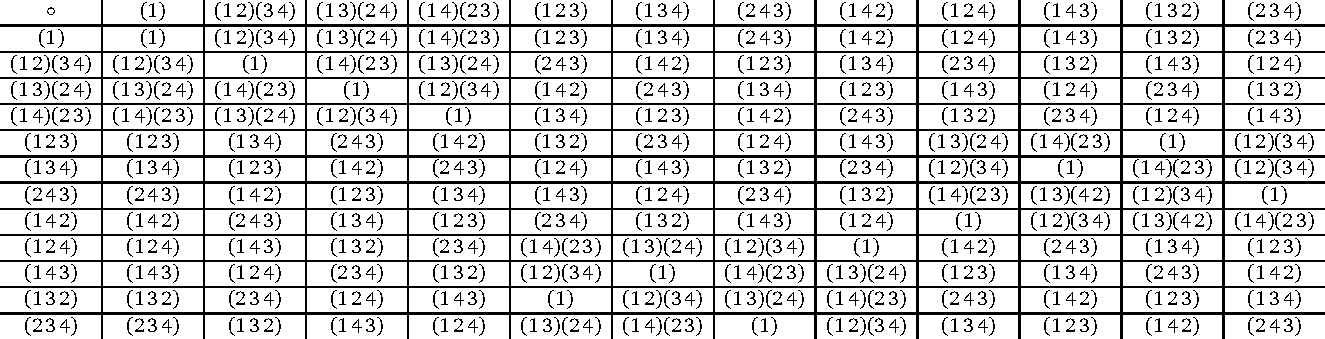
\includegraphics[width=\textwidth]{a4.eps}
\end{center}
\begin{problemparts}
  \item The set \(V=\{(1),(1\,2)(3\,4), (1\,3)(2\,4) , (1\,4)(2\,3)\} \) is a subgroup of \(A_4\). Explain how this fact can easily be verified using the above table.
  \item Write out the cosets of \(V\) in \(A_4\). (How big are they? How many of them are there?)
  \item Print out the above table, or make a screenshot and edit it in a drawing program. Assign a different color to each coset, and color each element in the table according to which coset it belongs to. What do you notice?
  \item Name the cosets \(X\), \(Y\), and \(Z\). Is there an obvious multiplication that makes the set \(\{X,Y,Z\}\) into a group? Draw a multiplication table.
  \item According to the ``obvious'' multiplication, if \(\alpha V\) and \(\beta V\) are cosets, what coset is their product \((\alpha V)(\beta V)\)?
\end{problemparts}
\end{problem}

\begin{definition}
Suppose that \(H\) is a subgroup of a group \(G\) and that \(a\) is some element of \(G\). Then \(Ha\) denotes the set \(\{ha \mid h \in H\}\), and is called a \textbf{right coset} of \(H\) in \(G\).
\end{definition}

\begin{problem}
Show, by giving an example of a group \(G\), a subgroup \(H\), and an element \(a\in G\), that \(Ha\) can be different from \(aH\). Is the statement, ``If \(x\in aH\) and \(y\in bH\), then \(xy \in (ab)H\)'' true, for all \(a,b\in G\) in your example?
\end{problem}

\begin{problem}\label{prob:kernorm}
Let \(\phi:G\longrightarrow H\) be a homomorphism of groups, and let \(K\) be the kernel of \(\phi\). Prove that \(aK = Ka \) for any \(a\in G\).
\end{problem}

\begin{problem}
Let \(H\) be a subgroup of a group \(G\) with the property that \(gH=Hg\) for all \(g\in G\). Let \(a,b\in G\). Prove that if \(x\in aH\) and \(y\in bH\), then \(xy \in (ab)H\).
\end{problem}

\section{Normal Subgroups}

\begin{definition}
If \(H\) is a subgroup of a group \(G\), we say that \(H\) is a \textbf{normal subgroup} if it satisfies the condition that \(gH = Hg\) for all \(g \in G\). In this case, we write \(H \lhd G\) and say ``\(H\)  is normal in \(G\).''
\end{definition}

For example, Problem~\ref{prob:a4comp} establishes that \(V \lhd A_4\). Problem~\ref{prob:kernorm} shows that kernels are normal subgroups. Of course, any subgroup of an abelian group is normal.

\begin{problem}\label{prob:normtest}
Let \(H\) be a subgroup of a group \(G\). Prove that \(H \lhd G\) if and only if the following condition holds: for all \(h\in H\) and for all \(g\in G\), \(ghg^{-1}\) is in \(H\).
\begin{annotation}
\endnote{Problem~\ref{prob:normtest} can be nicknamed ``the test for normality,'' but notice that it is reversible. Another way to state the converse of the test for normality is as a weak form of commutativity: If $H \lhd G$, then for any $g\in G$ and $h\in H$, $gh = h_1g$ for some $h_1 \in H$.}
\end{annotation}
\end{problem}

\begin{definition}
Suppose \(X\) and \(Y\) are subsets of a group \(G\). The set \(XY = \{xy \mid x\in X \mbox{ and } y\in Y\}\) is the \textbf{product} of the sets \(X\) and \(Y\). This product is also called ``set multiplication.''
\end{definition}

\begin{problem}\label{prob:cosmult}
Suppose that \(H\) is a normal subgroup of a group \(G\). Let \(a,b\in G\) and define \(X = aH\) and \(Y = bH\). Prove that \(XY = (ab)H\). (In other words, prove that the product of two cosets of a normal subgroup is another coset, and the representative of the product is the product of the representatives.)
\end{problem}

\begin{problem}
Give an example to show that the hypothesis that \(H\lhd G\)  is needed in Problem~\ref{prob:cosmult}. That is, find an example of a group and a subgroup where the product of two cosets fails to be a coset.
\end{problem}

\textbf{Notation:} Let \(H\) be a subgroup of a group \(G\). The set of all left cosets of \(H\) in \(G\) is denoted by \(G/H\). In other words, \(G/H = \{gH \mid g\in G\}\).

\begin{problem}
Let \(H\) be a normal subgroup of a group \(G\). Prove that the set \(G/H\)  is a group under coset multiplication.
\end{problem}

\begin{problem}
Let \(G = \mathbb{Z}_4\times \mathbb{Z}_6\), and let \(H\) be the cyclic subgroup generated by \((2,2)\). That is, \(H = \langle (2,2) \rangle \). Notice that \(H \lhd G\)  since \(G\) is abelian. Give the group table for \(G/H\). What well-known group is \(G/H\) isomorphic to?
\end{problem}

\section{Quotient Groups}

\begin{definition}
The group \(G/H\) is called the \textbf{quotient group} of \(G\) by \(H\), often pronounced ``\(G\) mod \(H\).''
\end{definition}

\begin{problem}
Let \(G\) be a group with \(H \lhd G\). Prove or disprove: If \(G\) is cyclic, then \(G/H\) is cyclic.
\end{problem}

\begin{problem}
Let \(G\) be a group with \(H \lhd G\). Prove or disprove: If \(G\) is abelian, then \(G/H\) is abelian.
\end{problem}

\begin{problem}
Let \(G\) be a group with \(H \lhd G\). Prove or disprove: If \(G/H\) is abelian, then \(G\) is abelian.
\end{problem}

\begin{problem}\label{prob:canonproj}
 In Problem~\ref{prob:kernorm}, you proved that all kernels are normal subgroups. Prove that all normal subgroups are kernels. That is, given a group \(G\) with a normal subgroup \(N \lhd G\), give a definition for a homomorphism \(\phi: G \longrightarrow G/N \) such that \(\mbox{Ker}(\phi)=N\), and show that the $\phi$ you define really is a homomorphism with this kernel.
\begin{annotation}
\endnote{The homomorphism defined in Problem~\ref{prob:canonproj} is called the ``canonical projection'' (or ``natural projection'').}
\end{annotation}
\end{problem}

\begin{problem}\label{prob:fit1}
Let \(\phi: G\longrightarrow H\) be a homomorphism of groups, and let \(K = \mbox{Ker}(\phi)\). In Problem~\ref{prob:kernorm}, you proved that \(K \lhd G\). Define a map \(\psi : G/K \longrightarrow H\) by the formula \(\psi(aK)=\phi(a)\). Prove that this map is \textbf{well defined}. That is, prove that it doesn't depend on the choice of representative for the coset \(aK\): Show that if \(aK = bK\), then \(\psi(aK)=\psi(bK)\).
\end{problem}

\begin{problem}
Prove that the map \(\psi\) defined in Problem~\ref{prob:fit1} is a homomorphism.
\end{problem}

\begin{problem}\label{prob:fit2}
Prove that the map \(\psi\) defined in Problem~\ref{prob:fit1} is one-to-one.  Conclude that if \(\phi: G\longrightarrow H\) is a homomorphism of groups, then  \(G/\Ker(\phi) \simeq \phi(G)\).
\begin{annotation}
\endnote{Problem \ref{prob:fit2} asks a lot of the students, as it is easy to confuse $\Ker(\phi)$ with $\Ker(\psi)$ when applying the kernel test.}
\end{annotation}
\end{problem}

\begin{problem}\label{prob:onefincyc}
Let $G = \langle a \rangle$, where $a$ has order $n$. Use the result of Problem~\ref{prob:fit2} and the homomorphism of Problem~\ref{prob:finitecyclic}
to prove that \(\mathbb{Z}/\langle n \rangle \simeq G\).
\end{problem}

Problem \ref{prob:onefincyc} establishes that there is only one finite cyclic group of every order, up to isomorphism.

\section{Isomorphism Theorems}\label{sec:isothms}

The result of Problem~\ref{prob:fit2} is extremely important: henceforth, we shall refer to it as the \textbf{First Isomorphism Theorem.}
Informally, it says that if you mod out by the kernel, you get a group that is isomorphic to the image. As a commutative diagram, the First Isomorphism Theorem is represented as follows.
\begin{center}
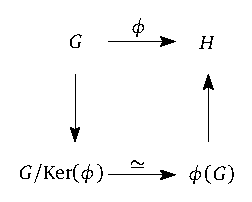
\includegraphics{fit.eps}
\end{center}

The downward map is the projection \(a \mapsto aK\), and the upward map is the inclusion \(a \mapsto a\). The map labeled as an isomorphism is the map considered in Problem~\ref{prob:fit2}.
\begin{annotation}
\endnote{Problems \ref{prob:hksubgroup}--\ref{prob:3it} will be challenging for students, who may benefit from some hints in advance.}
\end{annotation}

\begin{problem}\label{prob:hksubgroup}
Prove that if \(H\) and \(K\) are subgroups of a group \(G\), and \(K \lhd G\), then \(HK\)  is a subgroup of \(G\) and \(K \lhd HK\).
\end{problem}

\begin{problem}\label{prob:2it}
Let \(H\) and \(K\) be subgroups of a group \(G\) with \(K \lhd G\). Consider the map \[\phi : H \longrightarrow (HK)/K\] defined by \(\phi(a) = aK\). Use this map and the First Isomorphism Theorem to prove that \((HK)/K \simeq H/(H\cap K)\).
\begin{annotation}
\endnote{Problem \ref{prob:2it} is the Second Isomorphism Theorem.}
\end{annotation}
\end{problem}

\begin{problem}
Let \(H\) and \(K\) be normal subgroups of a group \(G\) with \(K \leq H\). Prove that \(H/K\) is a subgroup of \(G/K\), and furthermore, that \(H/K \lhd G/K\).
\end{problem}

\begin{problem}\label{prob:3it}
Let \(H\) and \(K\) be normal subgroups of a group \(G\) with \(K \leq H\). Consider the map \[\phi : G \longrightarrow (G/K)/(H/K)\] defined by \(\phi(g) = (gK)(H/K)\). Use this map and the First Isomorphism Theorem to prove that \(G/H \simeq (G/K)/(H/K)\).
\begin{annotation}
\endnote{Problem \ref{prob:3it} is the Third Isomorphism Theorem.}
\end{annotation}
\end{problem}

\chapter{Rings and Ideals}
To this point in the course, groups have been our main object of study, and we have established several key results about groups and learned some important techniques. Groups were defined with a somewhat minimal list of properties: associativity, identity, inverses. Given so few properties, it isn't surprising that most of the theorems we have been able to prove about groups have been fairly abstract.

Fortified with our newfound algebraic skills, we now move on to consider sets with additional properties, namely \emph{rings} and \emph{fields}. While the additional properties make these sets more complicated, the resulting theorems we will be able to prove will seem more like familiar facts about numbers. Historically, the ultimate goal of this study was to understand solutions of polynomial equations. While this remains our one of our goals (for this semester and the next), the resulting theory has been widely applied in other areas of mathematics.

\section{Rings}

\begin{definition}
A \textbf{ring} is a set \(R\) together with and addition operation \(+\) and a multiplication operation \(\cdot\) such that the following conditions hold.
\begin{enumerate}
  \item \(\langle  R, + \rangle \) is an abelian group with identity \(0 \in R\).
  \item Multiplication is associative.
  \item Multiplication distributes over addition: For all \(a,b,c\in R\), \(a(b+c)=ab+ac\) and \((b+c)a=ba+ca\).
\end{enumerate}
\end{definition}

We say that a ring is \textbf{commutative} if \(ab = ba\) for all \(a,b\in R\).
We call a ring a \textbf{ring with unity} if there is an element \(1\in R\) such that \(1\cdot a = a\cdot 1=a\) for all \(a\in R\).
In a ring with unity, the elements of a ring need not have multiplicative inverses. Elements that do have multiplicative inverses are called \textbf{units}.

\begin{problem}
Each set below is an example of a ring. For each example, determine whether it is commutative, whether it is a ring with unity, and if so, what the units are.
\begin{problemparts}
  \item \(\mathbb{Z}\), the integers under addition and multiplication.
  \item \(\mathbb{Z}_n\), the integers modulo \(n\) under addition and multiplication.
  \item \(M_2(\mathbb{R})\), the set of \(2\times 2\) matrices with entries in \(\mathbb{R}\). Addition is componentwise (add the corresponding entries), while multiplication is matrix multiplication.
  \item \(\mathbb{Q}[x]=\{a_0+a_1x+a_2x^2+\cdots+a_nx^n \mid n\in \{0,1,2,\ldots\}\mbox{ and } a_i\in \mathbb{Q}\}\), the set of polynomials in the variable \(x\) with rational coefficients. Add and multiply polynomials like you do in high school algebra: ``combine like terms'' and ``FOIL.''
\end{problemparts}
\end{problem}

The next four problems establish some basic properties of rings that we will use routinely subsequent work. The proofs use only the above properties in the definition of a ring, but at the same time they can be slightly tricky.
\begin{annotation}
\endnote{Consider providing hints for some of Problems~\ref{prob:zeromult}--\ref{prob:zeroring}.}
\end{annotation}

\begin{problem}\label{prob:zeromult}
Let \(R\) be a ring, and let \(r\in R\). Prove that \(0\cdot r = 0 = r\cdot 0\).
\end{problem}

\begin{problem}
Let \(R\) be a ring with unity, and let \(r\in R\). Let \(-1\) denote the additive inverse of \(1\). Prove that \(-1\cdot r = -r\). (That is, show that \(-1 \cdot r\) is the additive inverse of \(r\).)
\end{problem}

\begin{problem}
Let \(R\) be a ring with unity, and let \(-1\) denote the additive inverse of \(1\). Prove that \(-1 \cdot -1 = 1 \).
\end{problem}

\begin{problem}\label{prob:zeroring}
Let \(R\) be a ring with unity. Prove that if \(1=0\), then \(R = \{0\}\). (This ring is called the ``zero ring.'')
\end{problem}

Just as groups have subgroups and group homomorphisms, rings have \textbf{subrings} and \textbf{ring homomorphisms}.

\begin{problem}\label{prob:subringdef}
Without consulting any textbooks, the internet, or anyone else, make a guess at a definition of a \textbf{subring}. Find a nontrivial example of a subring that fits your definition.
\end{problem}

\begin{problem}\label{prob:ringhmmdef}
Without consulting any textbooks, the internet, or anyone else, make a guess at a definition of a \textbf{ring homomorphism}. Find a nontrivial example of a ring homomorphism that fits your definition.
\begin{annotation}
\endnote{Students will usually come up with the standard definitions, but before proceeding be sure that the class agrees on the results of Problems~\ref{prob:subringdef} and~\ref{prob:ringhmmdef}.}
\end{annotation}
\end{problem}

\section{Homomorphisms and Kernels}
As problems 94 and 95 illustrate, many of the definitions and examples associated with rings are natural extensions of those for groups. We won't necessarily restate them all, but here's one:

\begin{definition}
Suppose that \(R\) and \(S\) are rings, and that \(\phi : R \longrightarrow S\) is a ring homomorphism. The \textbf{kernel} of \(\phi\), denoted by \(\mbox{Ker}( \phi )\), is defined to be the
set \(\{r \in R \mid \phi(r) = 0 \} \), where \(0\) is the additive identity of \(S\).
\end{definition}

\begin{problem}
Let \(\mathbb{Z}[x]\)  be the ring of polynomials with integer coefficients. Fix \(a\in \mathbb{Z}\). It is easy to check that the map \(\epsilon_a : \mathbb{Z}[x] \longrightarrow \mathbb{Z}\) defined by \(\epsilon_a(p(x)) = p(a)\) is a ring homomorphism. Take this as given. The map \(\epsilon_a\) is called the \textbf{evaluation homomorphism}.
\begin{problemparts}
  \item Compute the kernel of \(\epsilon_0\).
  \item Compute the kernel of \(\epsilon_3\).
\end{problemparts}
\end{problem}

\begin{problem}\label{prob:ringkern}
Define \(\phi:\mathbb{Z}_5\longrightarrow \mathbb{Z}_5\) by \(\phi(n)=n^5\).
\begin{problemparts}
  \item Show that \(\phi\) is a homomorphism of rings.
  \item Compute \(\mbox{Ker}(\phi)\).
  \item Based on part (b), what do you conclude about \(\phi\)?
\begin{annotation}
\endnote{The following paragraph explains how students are supposed to know how to answer Problem~\ref{prob:ringkern}(c).}
\end{annotation}
\end{problemparts}
\end{problem}

Don't forget: If \(R\) is a ring, then \(\langle R, +\rangle\) is an abelian group. So any theorems you know about groups apply to \(R\) as an abelian group under addition. Beware, however, that theorems about groups do not apply to the multiplication in a ring. You can appeal to group theory to prove facts about the addition in a ring, but you still may have some work to do to prove corresponding facts about the ring's multiplication.

\begin{problem}\label{prob:ringimage}
Prove that the image of a ring homomorphism is a subring of the codomain. That is, if \(\phi: R \longrightarrow S\) is a ring homomorphism, and \(\phi(R) = \{\phi(r) \mid r\in R\}\), then \(\phi(R)\) is a subring of~\(S\).
\begin{annotation}
\endnote{Students will often prove more than they need to. That's fine. After they do, remind them that they could have used Problem~\ref{prob:imagesubgp} for the addition part of the proof of Problem~\ref{prob:ringimage}.}
\end{annotation}
\end{problem}

\begin{problem}\label{prob:idealprop}
Let \(\phi: R \longrightarrow S\) be a ring homomorphism, and let \(K = \mbox{Ker}(\phi)\).
\begin{problemparts}
  \item Explain why \(\langle K, + \rangle\) is a subgroup of \(\langle R, +\rangle \).
  \item Prove that, if \(k\in K\) and \(r \in R\), then \(kr \in K\) and \(rk \in K\).
\end{problemparts}
Explain how the result you just proved shows that \(K\) is a subring of \(R\), and in fact is a stronger condition.
\begin{annotation}
\endnote{As the subsequent paragraph makes clear, a nickname for the result in Problem~\ref{prob:idealprop} should be "kernels are ideals."}
\end{annotation}
\end{problem}

\section{Ideals}
In our study of groups, we found that the kernel \(K\) of a group homomorphism was a subgroup with an additional property: \(gK = Kg\) for all group elements \(g\). We defined a subgroup with this property to be a ``normal'' subgroup, and we saw how to use normal subgroups to construct quotient groups. In the same way, Problem~\ref{prob:idealprop} shows that the kernel of a ring homomorphism is a subring with some additional desirable properties; a set with these properties is called an \textbf{ideal}.

\begin{definition}
Let \(R\) be a ring. A subset \(I \subseteq R\) is called an \textbf{ideal} of \(R\) if it satisfies the following properties.
\begin{itemize}
  \item \(\langle I, +\rangle \) is a subgroup of \(\langle R, + \rangle \).
  \item For all \(r \in R\) and \(a \in I\), \(ra \in I\) and \(ar \in I\).
\end{itemize}
\end{definition}

This definition defines a ``two-sided ideal.'' It is possible to consider ``left ideals'' and ``right ideals'' which only satisfy one of the conditions \(ra \in I\) and \(ar \in I\), respectively. We will use the term ``ideal'' to refer to a two-sided ideal by default. Of course, in a commutative ring, you only have to check one of these conditions, since all ideals are two sided.

\begin{problem}
Let \(\mathbb{Z}[x]\) be the ring of polynomials in \(x\) with integer coefficients.
\begin{problemparts}
  \item Let \(I\) be the subset of \(\mathbb{Z}[x]\) consisting of polynomials with no constant term; that is, \(I = \{a_1x+a_2x^2+a_3x^3 + \cdots \mid a_i \in \mathbb{Z} \}\). Is \(I\) an ideal of \(\mathbb{Z}[x]\)? Prove or disprove.
  \item Let \(J\) be the subset of \(\mathbb{Z}[x]\) consisting of polynomials with only even degree terms; that is, \(J = \{a_0+a_2x^2+a_4x^4 + \cdots \mid a_i \in \mathbb{Z} \}\). Is \(J\) an ideal of \(\mathbb{Z}[x]\)? Prove or disprove.
\end{problemparts}
\end{problem}

\begin{problem}
Let \(R\) be the set of all real-valued functions on \(\mathbb{R}\). That is, \(R = \{ f \mid f : \mathbb{R}\longrightarrow \mathbb{R} \} \). Such functions can be added and multiplied \emph{pointwise:} If \(f\) and \(g\) are functions, then \(f+g\) and \(f\cdot g\) are functions defined by the formulas \((f+g)(x) = f(x)+g(x)\) and \((f\cdot g)(x) = f(x)g(x) \). With these operations, \(R\) is a commutative ring.
\begin{problemparts}
  \item Prove that the set \(I = \{ f \in R \mid f(3)=0\} \) is an ideal of \(R\).
  \item Prove that the set \(J = \{ f \in R \mid f(3)=1\} \) is not an ideal of \(R\).
\end{problemparts}
\end{problem}

\begin{problem}\label{prob:noncomring}
Let \(I\) be the subset of \(M_2(\mathbb{R})\) consisting of matrices whose second column is zero. That is, \[I=\left\{ \begin{bmatrix}a & 0 \\ b & 0\end{bmatrix} \mid a,b\in \mathbb{R}\right\}\]
Prove that \(I\) is a left ideal but it isn't a right ideal.
\begin{annotation}
\endnote{Problem~\ref{prob:noncomring} provides one of our few examples of non-commutative rings. Most of the subsequent material will involve commutative rings.}
\end{annotation}
\end{problem}

\begin{problem}
Let \(R\) be a commutative ring. Fix an element \(a \in R\). Define the set \(I \subseteq R\) by \(I = \{ ra \mid r\in R\}\). Prove that \(I\) is an ideal of \(R\).
\end{problem}

\textbf{Definition:} If \(R\) is a commutative ring and \(a\in R\), then the set \(\{ra \mid r\in R\}\) is called the \textbf{principal ideal} generated by \(a\). This ideal is denoted by \((a)\).

\begin{problem}
Find all (distinct) principal ideals of the ring \(\mathbb{Z}_{12}\). Make a conjecture that generalizes this problem to \(\mathbb{Z}_n\).
\end{problem}

\chapter{Quotient Rings}

\begin{problem}
Let \(I\) be an ideal of a ring \(R\) with unity. Prove that if \(1\in I\), then \(I=R\). (In other words, prove that no proper ideal can contain the multiplicative identity.)
\end{problem}

\section{Cosets}

Let \(I\) be an ideal of a ring \(R\). For any \(r\in R\), the set \(r+I = \{r+i \mid i \in I\}\) is called a \textbf{coset} of \(I\) in \(R\). The set of all cosets of \(I\) in \(R\) is denoted by \(R/I\). If \(X\) and \(Y\) are subsets of a ring, we define ``set addition'' by letting the \textbf{sum} \(X+Y\) be the set \(\{x+y \mid x\in X \mbox{ and } y\in Y\}\).
These definitions are identical to the corresponding definitions for a group; the only difference is that we are using additive notation instead of multiplicative notation.

\begin{problem}
Let \(I\) be an ideal of a ring \(R\). Explain why \(\langle I, +\rangle\) is a normal subgroup of \(\langle R, + \rangle \). Which problems (that we have already proved) establish the following facts?
\begin{problemparts}
  \item The cosets of \(I\) in \(R\) partition \(R\).
  \item The cosets of \(I\) in \(R\) all have the same size (or cardinality).
\begin{annotation}
\endnote{We have only talked about the ``size'' of finite sets, and we choose not to introduce notions of cardinality of infinite sets to streamline the presentation. If students do not learn about cardinality in previous classes, be prepared to give a short explanation.}
\end{annotation}
  \item If \(R\) is finite, then \(\lvert I \rvert \) divides \(\lvert R \rvert\).
  \item For all \(r,s \in R\), \((r+I)+(s+I) = (r+s) + I\).
  \item The set \(R/I\) is a group under coset addition.
\end{problemparts}
\end{problem}

\begin{problem}\label{prob:ringset}
If \(X\) and \(Y\) are subsets of a ring, we could define ``set multiplication'' by letting the product \(XY\) be the set \(\{xy \mid x\in X \mbox{ and } y\in Y\}\), as we did with groups. Unfortunately, this notion of multiplication fails on the cosets of a ring; give an example to show that it fails. In other words, find an example of a ring \(R\), an ideal \(I\), and cosets \(a+I\) and \(b+I\) such that the set  \(\{xy \mid x\in a+I \mbox{ and } y\in b+I\}\) is not a coset of \(I\) in \(R\).
\end{problem}

\section{Constructing Quotient Rings}
We now know that the set \(R/I\) is an abelian group; we would like to make it into a ring. However, in light of Problem~\ref{prob:ringset}, we need a different notion of what it means to multiply the cosets of a ring.

\begin{definition}
Let \(I\) be an ideal of a ring \(R\), and let \(a,b \in R\). The \textbf{coset product} of \(a+I\) and \(b+I\) is the coset \(ab+I\). That is, \( (a+I)(b+I) = ab +I\).
\end{definition}

The next problem has you check that the coset product is well defined.
\begin{annotation}
\endnote{The notion of being ``well defined'' was introduced in Problem~\ref{prob:fit1}, but may need some amplification here.}
\end{annotation}

\begin{problem}
Let \(I\) be an ideal of a ring \(R\), and let \(a,b \in R\). Prove that the coset product does not depend on the choice of coset representatives. That is, prove that if \(a + I = x +I\) and \(b +I = y+I\), then \(ab + I = xy +I\).
\end{problem}

\begin{problem}
Prove that the set \(R/I\) is a ring under coset addition and coset multiplication.
\end{problem}

\section{Isomorphisms}

\begin{problem}
The ring \(\mathbb{Z}_2[x]/(x^2)\) has four elements. List them, and make an addition and multiplication table. Is this ring isomorphic to any other rings that you have seen before?
\end{problem}

\begin{problem}
Review your solution to Problem~\ref{prob:fit2} and the discussion at the beginning of Section~\ref{sec:isothms}. Then state and prove the First Isomorphism Theorem for rings.
\begin{annotation}
\endnote{When translating the First Isomorphism Theorem from groups to rings, students may need to be reminded that cosets are being written in additive notation.}
\end{annotation}
\end{problem}

\begin{problem}
Let \(R\) be a ring. Prove that the set \(\{0\}\) is an ideal of \(R\), and that \(R/\{0\} \simeq R\).
\end{problem}

\begin{problem}
 Let \(R\) be a ring with unity. Prove that \(R\) has a subring that is isomorphic to either \(\mathbb{Z}\) or \(\mathbb{Z}/ (n)\) for some \(n\).
\end{problem}

\begin{problem}\label{prob:cxnumintro}
Let \(\mathbb{R}\) denote the ring of real numbers, let \(\mathbb{R}[x]\) be the ring of polynomials with real coefficients, let \( (x^2+1) \) be the principal ideal generated by \(x^2+1\),  and let \(\mathbb{C}\) denote the ring of complex numbers. Prove that \(\mathbb{R}[x]/( x^2+1) \simeq \mathbb{C} \).
\begin{annotation}
\endnote{A rigorous proof of Problem~\ref{prob:cxnumintro} requires more development. We deal with some of the issues in later chapters. Students will need to use their prior knowledge about real polynomials to justify their answer. This can lead to a discussion about how to prove these facts in more generality, as a transition to upcoming material.}
\end{annotation}
\end{problem}

\chapter{Divisibility}
In a ring, you can add, subtract, and multiply, but you can't divide, in general. However, there are certain abstract properties that approach the idea of division in a ring, and the extent to which a ring has these properties characterizes different types of rings. For simplicity in what follows, we will mainly consider the case of commutative rings with unity, though some of these ideas can be stated in more generality.

\begin{definition}
We say that a commutative ring \(R\) has the \textbf{cancellation property} if, for all \(a, b, r \in R\) with \(r\neq 0\), \(ar = br\) implies \(a = b\).
\end{definition}

\begin{definition}
A nonzero element \(a\) in a commutative ring \(R\) is called a \textbf{divisor of zero} (or ``zero divisor'') if there exists some nonzero \(r \in R\) such that \(ar = 0\).
\end{definition}

\begin{problem}
Let \(R\) be a commutative ring. Prove that, if \(R\) has the cancellation property, then \(R\) has no divisors of zero.
\end{problem}

\begin{problem}
Let \(R\) be a commutative ring. Prove that, if \(R\) has no divisors of zero, then \(R\) has the cancellation property.
\end{problem}

\section{Integral Domains and Fields}

\begin{definition}
A commutative ring with unity is called an \textbf{integral domain} if it satisfies the cancellation property (or equivalently, if it has no divisors of zero).
\end{definition}

For example, \(\mathbb{Z}\) is an integral domain, but \(\mathbb{Z}_6\) isn't, because \(2\) is a zero divisor in \(\mathbb{Z}_6\).

\begin{definition}
A commutative ring with unity is called a \textbf{field} if every nonzero element has a multiplicative inverse.
\end{definition}

For example, \(\mathbb{Q}\) is a field.
\begin{annotation}
\endnote{Now might also be a good time to introduce an example of a finite field (e.g., $\ZZ_3$), where the existence of inverses can be checked easily for each nonzero element.}
\end{annotation}

\begin{problem}
Prove that every field is an integral domain.
\end{problem}

\begin{problem}\label{prob:noideal}
Prove that a field has no nontrivial proper ideals. Use this fact to explain why any nontrivial homomorphism \(\phi: F \longrightarrow E\) of fields must be one-to-one.
\begin{annotation}
\endnote{Students often need reassurance that earlier material on groups can be applied. They may need help remembering that injectivity is a set-theoretic property, ideals are abelian subgroups, and a homomorphism of fields is a homomorphism of abelian groups, so they can use results like Problem~\ref{prob:kernelsubgp} and its consequences.}
\end{annotation}
\end{problem}

\begin{definition}
Let \(p(x) \in R[x]\) be the polynomial \(p(x) = a_0 + a_1x + a_2x^2 + \cdots + a_nx^n \). The \textbf{degree} of \(p(x)\) is the greatest integer \(k\) such that \(a_k \neq 0\). Notation: \(\mbox{deg} (p) = k\).
\end{definition}

Every polynomial has a degree, except for the zero polynomial. If \(\mbox{deg}(p)=0\), then \(p(x)=c\) for some nonzero constant \(c\in R\).

\begin{problem}
Let \(R\) be an integral domain, and let \(p(x),q(x) \in R[x]\) be nonzero polynomials. Prove that \(\mbox{deg}(pq) = \mbox{deg}(p)+\mbox{deg}(q)\). Use this fact to explain why \(R[x]\) must also be an integral domain.
\end{problem}

\section{The Division Algorithm}
When you learned the algorithm for long division in grade school, your teacher probably didn't mention the issues of \emph{existence} and \emph{uniqueness}. The process always terminated in a result, and every question only had one answer. These issues become more murky as we consider division of polynomials in a more abstract setting.

\begin{theorem}[The Division Algorithm]
Let \(R\) be a commutative ring with unity, and let \(f(x),g(x)\in R[x]\). Furthermore, suppose that
\begin{align*}
f(x) &= a_0 + a_1x +a_2x^2 + \cdots + a_m x^m \\
g(x) &= b_0 + b_1x +b_2x^2 + \cdots + b_n x^n
\end{align*}
such that $b_n$ is a unit in \(R\). Then there are polynomials \(q(x)\) and \(r(x)\) in \(R[x]\) (called the ``quotient'' and ``remainder'') such that
\[ f(x) = q(x)g(x) + r(x) \]
and either \(r(x) = 0\) or \(\mbox{deg}(r) < \mbox{deg}(g) \).
\end{theorem}

\begin{problem}
Find polynomials \(q(x)\) and \(r(x)\) guaranteed by the division algorithm in \(\mathbb{Z}[x]\) when \(f(x) = 4x^3 + 3x^2 + 2x + 1\) and \(g(x)=x^2 - x - 1 \). Is the answer uniquely determined?
\end{problem}

Problems \ref{prob:daproof1}--\ref{prob:daproof3} will lead you through a proof of the division algorithm. Let \(f\), \(g\), and \(R\) be as in the hypotheses of the theorem.
\begin{annotation}
\endnote{Problems \ref{prob:daproof1}--\ref{prob:daproof3} give a highly scaffolded approach to the proof of the Division Algorithm. The steps may be ``locally clear'' to students, but they may need some help seeing the big picture. Informally, the set $X$ plays the role of ``possible remainders,'' and the proof confirms that one of its elements is the required remainder.}
\end{annotation}

\begin{problem}\label{prob:daproof1}
Let \(X = \{f(x)-g(x)p(x) \mid p(x) \in R[x] \}\). Suppose that \(0 \in X\). Show that the conclusion of the division algorithm (i.e., the last sentence) follows in this case.
\end{problem}

\begin{problem}\label{prob:daproof2}
Let \(X\) be as in Problem~\ref{prob:daproof1}, and suppose that \(0 \not\in X\). Then every element of \(X\) has a degree. Let \(r(x)\) be an element of minimal degree in \(X\), and let $l = \mbox{deg}(r)$. Then \(f(x) = q(x)g(x) + r(x)\) for some \(q(x)\in R[x]\), so we just need to show that \(\mbox{deg}(r) < \mbox{deg}(g) \). Suppose to the contrary that \(r(x) = c_0 + c_1x + c_2x^2 + \cdots + c_lx^l\) with \(c_l\neq 0\) and \(l \geq n\). Show that the degree of the polynomial \(r(x)-b_n^{-1}c_lx^{l-n}g(x)\) is less than $l$.
\end{problem}

\begin{problem}\label{prob:daproof3}
Let \(r\) and \(X\) be as in  Problem~\ref{prob:daproof2}, so $r(x) = f(x) - q(x)g(x)$. Substitute the formula $f(x) - q(x)g(x)$ for $r(x)$ to show that the polynomial \(r(x)-b_n^{-1}c_lx^{l-n}g(x)\) is in \(X\). Explain why this conclusion results in a contradiction.
\begin{annotation}
\endnote{The polynomial considered in Problems~\ref{prob:daproof3} and \ref{prob:daproof2} is an example of ``pulling a rabbit out of a hat.'' If time permits, consider discussion how this polynomial might have been motivated.}
\end{annotation}
\end{problem}

\begin{problem}\label{prob:divalgunique}
Suppose, in addition to the hypotheses of the division algorithm, that \(R\) is an integral domain. Prove that the polynomials \(q(x)\) and \(r(x)\) are uniquely determined.
\end{problem}

\begin{problem}
Show that if $R$ is not an integral domain, then the uniqueness property of Problem~\ref{prob:divalgunique} can fail. In particular, show that in \(\mathbb{Z}_4[x]\), there are polynomials \(q_1(x)\), \(q_2(x)\), \(r_1(x)\), \(r_2(x)\), and \(g(x)\) with \(\mbox{deg}(r_1)<\mbox{deg}(g)\) and \(\mbox{deg}(r_2)<\mbox{deg}(g)\) and such that \(q_1(x) \neq q_2(x)\) and \(r_1(x) \neq r_2(x)\), but such that \(q_1(x)g(x) +r_1(x) = q_2(x)g(x)+r_2(x)\).
\end{problem}

\begin{problem}\label{prob:fieldprin}
Let \(F\) be a field. Use the division algorithm to prove that every ideal of \(F[x]\) is a principal ideal. That is, prove that if \(I\) is an ideal of \(F[x]\), then there is some generating polynomial \(p(x) \in F[x]\) such that \(I = \left(p(x)\right)\).
\begin{annotation}
\endnote{Going forward, the result of Problem~\ref{prob:fieldprin} is one of the most important applications of the division algorithm. Later we will introduce the term ``principal ideal domain,'' but this term could also be previewed at this point.}
\end{annotation}
\end{problem}

\textbf{Terminology:} The highest-degree term of a polynomial is called its \textbf{leading term}. A polynomial is \textbf{monic} if its leading term has coefficient \(1\).

\begin{problem}
Let \(F\) be a field, and let \((p(x))\) be an ideal of \(F[x]\). Prove that \((p(x))\) = \((m(x))\) for some monic polynomial \(m(x)\).
\end{problem}

\begin{problem}
Suppose that \(R\) is a commutative ring with unity, and that the only ideals of \(R\) are \(R\) and \(\{0\}\). Prove that \(R\) is a field. (This is the converse of Problem~\ref{prob:noideal}.)
\end{problem}

\begin{problem}
Let \(F\) be a field. Prove that the only units of \(F[x]\) are the nonzero constants. (More generally, if \(R\) is an integral domain, then any unit of \(R[x]\) must have degree zero.)
\end{problem}

\textbf{Notation and Terminology:} The set of all \textbf{multiples} of \(a\) in a ring \(R\) is denoted by \((a) = \{ra \mid r\in R\}\) and is called the \textbf{principal ideal generated by} \(a\). Similarly, let \(a_1, a_2, \ldots, a_n \in R\), a commutative ring. The set of all \textbf{linear combinations} of the \(a_i\)'s is denoted by \((a_1, a_2, \ldots, a_n) = \{r_1a_1 + r_2a_2 + \cdots + r_na_n \mid r_i \in R\} \). The next problem will show that this set is also an ideal, called the ideal \textbf{generated} by \(a_1, a_2, \ldots, a_n\).

\begin{problem}
Let \(a_1, a_2, \ldots, a_n \in R\), a commutative ring. Prove that \((a_1, a_2, \ldots, a_n)\) is an ideal of \(R\).
\end{problem}

\begin{problem}\label{prob:notprinid}
In \(\mathbb{Z}[x]\), prove that \((x,2) \neq (x+2)\), \((x,2) \neq (x)\), and \((x,2) \neq (2)\).
\begin{annotation}
\endnote{The point of Problem~\ref{prob:notprinid} is to introduce an ideal that is not a principal ideal. This problem also illustrates the need for the field hypothesis in Problem~\ref{prob:fieldprin}.}
\end{annotation}
\end{problem}

\section{Greatest Common Divisor}
\begin{definition}
Let \(a,b\in R\), a commutative ring. We say that \(a\) \textbf{divides} \(b\), written \(a\mid b\),  if \(ar = b\) for some \(r \in R\). Alternatively, we also say that \(b\) is a \textbf{multiple} of \(a\).
\end{definition}

\begin{problem}
Let \(a,b,c\in R\), a commutative ring. Prove that if \(a\mid b\) and \(b\mid c\), then \(a \mid c\). (This shows that the ``\(\mid\)'' relation is \textbf{transitive}.)
\end{problem}

\begin{problem}
Let \(a,b\in R\), an integral domain. Suppose that \(a \mid b\) and \(b \mid a\). Show that \(a = ub\), where \(u\) is a unit in \(R\).
\end{problem}

\begin{definition}
Let \(R\) be an integral domain, and let \(f(x),g(x)\in R[x]\). The \textbf{greatest common divisor} of \(f(x)\) and \(g(x)\) is a polynomial \(d(x)\) that satisfies the following three properties.
\begin{enumerate}
  \item \(d(x) \mid f(x)\) and \(d(x) \mid g(x)\).
  \item If \(c(x)\in R[x]\) is a polynomial such that \(c(x) \mid f(x)\) and \(c(x) \mid g(x)\), then \(c(x) \mid d(x)\).
  \item \(d(x)\) is monic.
\end{enumerate}
In this case we write \(d(x) = \mbox{gcd}(f(x),g(x))\).
\end{definition}

\emph{Warning:} Some books omit condition 3 when giving this definition. We include it for convenience, because our focus later will be on polynomial rings over fields. You may notice some discrepancies when dealing with polynomial rings over rings that aren't fields. For example, according to our definition, in \(\mathbb{Z}[x]\), \(\text{gcd}(3x+1, 6x+2) = 1\), while other definitions would allow \(3x+1\) as the common divisor.

The use of the definite article ``the'' in this definition suggests that the greatest common divisor of two polynomials, if it exists, is uniquely determined. We still need to prove this assertion.

\begin{problem}
Let \(R\) be an integral domain, and let \(f(x),g(x)\in R[x]\). Suppose that \(f(x)\) and \(g(x)\) have a greatest common divisor.  Prove that it is unique.
\end{problem}

\begin{problem}
Find the greatest common divisor of \(x^2-x-6\) and \(x^3+x^2-3x-2\) in \(\mathbb{Q}[x]\).
\end{problem}

\begin{problem}\label{prob:relprimegcd}
Let \(a(x), b(x), f(x), g(x) \in R[x]\), where \(R\) is an integral domain. Suppose that \(a(x)f(x)+b(x)g(x) = 1\). Prove that \(\mbox{gcd}(f(x),g(x))=1\). (We say that such polynomials \(f(x)\) and \(g(x)\) are \textbf{relatively prime}.)
\begin{annotation}
\endnote{I tell the students that it is OK to omit the $x$'s in the proof of~\ref{prob:relprimegcd} and similar proofs (e.g., write $af + bg = 1$ in place of \(a(x)f(x)+b(x)g(x) = 1\)). Doing so makes the calculations easier to follow for some.}
\end{annotation}
\end{problem}

\begin{theorem}\label{thm:gcdlincomb}
Let \(F\) be a field, and let \(f(x)\) and \(g(x)\) be nonzero polynomials in \(F[x]\). Then there exist polynomials \(a(x)\) and \(b(x)\) in \(F[x]\) such that \[d(x) = a(x)f(x) + b(x)g(x)\]
is the greatest common divisor of \(f(x)\) and \(g(x)\).
\begin{annotation}
\endnote{A nickname for Theorem \ref{thm:gcdlincomb} could be ``the gcd is a linear combination.'' This important theorem also establishes the existence of a gcd in the case of polynomial rings over fields.}
\end{annotation}
\end{theorem}

\begin{problem}\label{prob:gcdlincomb}
The following statements establish a proof of the above theorem. Give a reason for each statement (cite previous problems, or give a brief justification).
\begin{annotation}
\endnote{Problem \ref{prob:gcdlincomb} gives students the opportunity to step back and see the big picture of the results in this chapter. It also is worth discussing which parts of the proof use the hypothesis that $F$ is a field.}
\end{annotation}
\begin{problemparts}
  \item The set \(I\) of all linear combinations of \(f(x)\) and \(g(x)\) is an ideal of \(F[x]\).
  \item The ideal \(I\) can be written as \(I = (d(x))\) for some monic polynomial \(d(x)\).
  \item There exist polynomials \(a(x)\) and \(b(x)\) in \(F[x]\) such that \(d(x) = a(x)f(x) + b(x)g(x)\).
  \item The polynomial \(d(x)\) is a common divisor of \(f(x)\) and \(g(x)\).
  \item If \(c(x)\in F[x]\) is a polynomial such that \(c(x) \mid f(x)\) and \(c(x) \mid g(x)\), then \(c(x) \mid d(x)\).
\end{problemparts}
\end{problem}

\begin{problem}\label{prob:unitquotring}
Let \(f(x)\) and \(g(x)\) be nonzero polynomials in \(F[x]\), where \(F\) is a field. Let \(I = (f(x))\). Suppose that \(g(x) + I\) is a unit in the quotient ring \(F[x]/I\). Prove that \(f(x)\) and \(g(x)\) are relatively prime.
\begin{annotation}
\endnote{Problems \ref{prob:unitquotring}--\ref{prob:findinvqr} return to the topic quotient rings for the first time in this chapter, so students may need to be reminded about some facts from Chapter 7.}
\end{annotation}
\end{problem}

\begin{problem}\label{prob:unitquotring2}
Let \(f(x)\) and \(g(x)\) be nonzero polynomials in \(F[x]\), where \(F\) is a field. Let \(I = (f(x))\). Suppose that \(f(x)\) and \(g(x)\) are relatively prime. Prove that \(g(x) + I\) is a unit in the ring \(F[x]/I\).
\end{problem}

\begin{problem}\label{prob:findinvqr}
Let \(I = (x^2+x+1)\) in \(\mathbb{Q}[x]\). Find the multiplicative inverse of \(x+1 +I\) in \(\mathbb{Q}[x]/I\), or explain why no such inverse exists.
\end{problem}

\section{The Euclidean Algorithm}

Euclid's Elements (300 BC) describe a procedure for computing the greatest common divisor of two numbers. Remarkably, this procedure works in polynomial rings over fields. In the next eight problems we will prove that it produces the greatest common divisor, and also that it gives the polynomials \(a(x)\) and \(b(x)\) to express \(\mbox{gcd}(f(x),g(x))\) as a linear combination \(a(x)f(x) + b(x)g(x)\).

The idea is to repeat the division algorithm: Given polynomials \(f(x)\) and \(g(x)\) in \(F[x]\), make the following sequence of calculations, continuing until the remainder of the division problem is zero.
\begin{align*}
f(x) & = q_1(x)g(x) + r_1(x) && \text{where } \mbox{deg}(r_1)<\mbox{deg}(g) \\
g(x) & = q_2(x)r_1(x) + r_2(x) && \text{where } \mbox{deg}(r_2)<\mbox{deg}(r_1) \\
r_1(x) & = q_3(x)r_2(x) + r_3(x) && \text{where } \mbox{deg}(r_3)<\mbox{deg}(r_2) \\
r_2(x) & = q_4(x)r_3(x) + r_4(x) && \text{where } \mbox{deg}(r_4)<\mbox{deg}(r_3) \\
\text{etc.}\ldots \\
r_{k-2}(x) & = q_k(x)r_{k-1}(x) + r_k(x) && \text{where } \mbox{deg}(r_k)<\mbox{deg}(r_{k-1}) \\
r_{k-1}(x) & = q_{k+1}(x)r_k(x) && \text{where } r_{k+1}(x) = 0
\end{align*}

\begin{problem}
Apply the Euclidean algorithm to the polynomials \(f(x) = x^4+x^3+x^2+x+1\) and \(g(x)=x^2+1\) in \(\mathbb{Q}[x]\). Why must this procedure always terminate?
\end{problem}

\begin{problem}\label{prob:backsub1}
Suppose that you carry out the Euclidean algorithm on some polynomials \(f(x)\) and \(g(x)\) in \(F[x]\), a polynomial ring over a field, and that after three steps you find that \(r_3(x) = u\), a constant polynomial in \(F[x]\). Find polynomials \(a(x)\) and \(b(x)\) (in terms of \(u\), the \(q_i\)'s and the \(r_i\)'s) such that \(a(x)f(x)+b(x)g(x) = 1\).
\begin{annotation}
\endnote{Rather than spending time on the algorithm for back substitution, Problem~\ref{prob:backsub1} encourages students to come up with an \textit{ad hoc} method. Problem~\ref{prob:backsub2} revisits this procedure. The goal is for students to see that the linear combination can be recovered, without dwelling too much on the computational details.}
\end{annotation}
\end{problem}

\begin{problem}\label{prob:z3euclid}
It is easy to check that the ring $\ZZ_3$ is a field. Carry out the Euclidean algorithm using the polynomials \(f(x)=x^4+2x^3+2x+1\) and \(g(x) = x^3+2x^2+x+2\) in \(\mathbb{Z}_3[x]\).
\end{problem}

Problems \ref{prob:eucalgpf1}--\ref{prob:eucalgpf4} will lead you through a proof that the Euclidean algorithm computes the greatest common divisor.

\begin{problem}\label{prob:eucalgpf1}
Let \(I = (f(x),g(x))\) be the ideal of \(F[x]\) consisting of all linear combinations of \(f(x)\) and \(g(x)\). Prove that, in the Euclidean algorithm, the remainders
$$r_1(x), r_2(x), r_3(x), \ldots , r_k(x)$$
are all elements of \(I\).
\end{problem}

\begin{problem}
Let \(f(x)\) and \(g(x)\) in \(F[x]\), a polynomial ring over a field, and suppose that \(c(x)\) is a common divisor of \(f(x)\) and \(g(x)\). Prove that \(c(x)\) divides all of the remainders \(r_1(x), r_2(x), r_3(x), \ldots , r_k(x)\) produced by the Euclidean algorithm.
\end{problem}

\begin{problem}
Let \(f(x)\) and \(g(x)\) in \(F[x]\), a polynomial ring over a field, and suppose that \(r_1(x), r_2(x), r_3(x), \ldots , r_k(x)\)  are the remainders produced by the Euclidean algorithm. Prove that \(r_k(x)\) divides all of the other remainders.
\end{problem}

\begin{problem}\label{prob:eucalgpf4}
Let \(f(x)\) and \(g(x)\) in \(F[x]\), a polynomial ring over a field, and suppose that \(r_k(x)\) is the last nonzero remainder produced by the Euclidean algorithm. Prove that \(r_k(x) = ud(x)\), where \(u \in F\) and \(d(x)=\mbox{gcd}(f(x),g(x))\).
\begin{annotation}
\endnote{Nickname for Problem \ref{prob:eucalgpf4}: ``The last nonzero remainder is the gcd,'' up to a unit multiple.}
\end{annotation}
\end{problem}


\begin{problem}\label{prob:backsub2}
Revisit Problem \ref{prob:z3euclid}. Write the greatest common divisor of \(f(x)=x^4+2x^3+2x+1\) and \(g(x) = x^3+2x^2+x+2\) in \(\mathbb{Z}_3[x]\) as a linear combination of \(f(x)\) and \(g(x)\). Is \(g(x)+(f(x))\) a unit in \(\mathbb{Z}_3[x]/(f(x))\)?
\end{problem}

\chapter{Prime Ideals and Maximal Ideals}

Historically, the development of modern abstract algebra was motivated by the study of the solutions to polynomial equations with integer coefficients. Solutions to quadratic equations were largely understood by Hindu mathematicians in the 7th century and Arab mathematicians in the 9th century, and special cases were known to the ancient Greeks and Babylonians. However, the general situation for higher-degree polynomials was not understood until the 19th century, and the important theorems rely on modern group theory as well as ring and field theory.
\begin{annotation}
\endnote{The important result in this chapter is Problem~\ref{prob:fieldconstruction}. If time is running short near the end of the semester, much of the material on prime and maximal ideals in this chapter can be skipped, and a plausibility argument for Problem~\ref{prob:fieldconstruction} can be given using Problem~\ref{prob:unitquotring2}. However, is important not to skip the construction of finite fields and extension fields of~$\QQ$.}
\end{annotation}

\section{Roots of Polynomials}

\begin{definition}
Let \(p(x) \in R[x]\), where \(R\) is a commutative ring. An element \(a \in R\) is called a \textbf{root} of \(p(x)\) if \(p(a) = 0\).
\end{definition}

\begin{problem}
Let \(f(x) \in F[x] \), where \(F\) is a field. Let \(a \in F\), and let \(r(x)\) be the remainder of the division algorithm applied to \(f(x)\) and \(g(x) = x-a\). Show that \(r(x) = f(a)\).
\end{problem}

\begin{problem}
Let \(f(x) \in F[x] \), where \(F\) is a field, and let \(a\in F\). Prove that \(a\) is a root of \(f(x)\) if and only if \((x-a) \mid f(x) \).
\end{problem}

\begin{problem}
Explain why a polynomial of degree \(n\) over a field \(F\) can have at most \(n\) distinct roots in \(F\).
\end{problem}

\begin{problem}
Find an example of a commutative ring in which the polynomial $x^2-1$ has more than two distinct roots.
\end{problem}

\begin{definition}
Let \(F\) be a field. A non-constant polynomial \(f(x)\in F[x]\) is called \textbf{reducible} over \(F\) if it can be factored into two polynomials of lower degree. That is, if there exist \(p(x)\) and \(q(x)\) with \(\text{deg}(p)<\text{deg}(f)\) and \(\text{deg}(q)<\text{deg}(f)\) and \(f(x)=p(x)q(x)\). A non-constant polynomial is called \textbf{irreducible} over \(F\) if it is not reducible over \(F\).
\end{definition}

For example, \(x^2+1\) is irreducible over \(\mathbb{Q}\), but this polynomial is reducible over \(\mathbb{C}\) since \(x^2+1 = (x-i)(x+i)\). The polynomial \(3x+6\) is irreducible over \(\mathbb{Q}\) (and over \(\mathbb{C}\)) because its only factorization is \(3x+6 = (3)(x+2)\), but these factors are not both of lower degree.

\begin{problem}\label{prob:deg2or3irr}
Let \(F\) be a field, and let \(f(x)\in F[x]\) be a polynomial of degree 2 or 3. Prove that \(f(x)\) is reducible over \(F\) if and only if \(f(x)\) has a root in \(F\).
\end{problem}

\begin{problem}
Give a counterexample to show that the conclusion of Problem~\ref{prob:deg2or3irr} does not hold for polynomials of degree 4 (or higher), in general.
\end{problem}

\section{Prime Ideals}
Proposition 30 of Book VII of Euclid's Elements says, ``If two numbers, multiplied by one another make some number, and any prime number measures the product, then it also measures one of the original numbers.'' This basic number-theoretical property, known as \emph{Euclid's Lemma,} can be stated in modern language as follows: If a prime number \(p\) divides a product \(ab\), then \(p\mid a\) or \(p \mid b\). The next definition is an abstraction of this basic fact.

\begin{definition}
Let \(I\) be an ideal of a commutative ring \(R\). Then \(I\) is a \textbf{prime ideal} if it is a proper ideal and, for any \(a,b\in R\), \(ab \in I\) implies \(a \in I\) or \(b \in I\).
\end{definition}

\begin{problem}
In the ring \(\mathbb{Z}\), show that \((7)\) is a prime ideal, but \((6)\) is not a prime ideal.
\end{problem}

\begin{problem}
Prove that if \(I\) is a prime ideal of a commutative ring \(R\) with unity, then \(R/I\) is an integral domain.
\end{problem}

\begin{problem}
Let \(I\) be an ideal of a commutative ring \(R\). Prove that if \(R/I\) is an integral domain, then \(I\) is a prime ideal.
\end{problem}

\begin{problem}
Let \(F\) be a field, and suppose that \(p(x) \in F[x]\) is a reducible polynomial. Show that \((p(x))\) is not a prime ideal of \(F[x]\).
\end{problem}

\begin{problem}
Prove \emph{Euclid's lemma} for polynomials: Let \(F\) be a field, and suppose that \(p(x)\in F[x]\) is irreducible. Prove that if \(p(x) \mid a(x)b(x)\) for some \(a(x),b(x)\in F[x]\), then \(p(x) \mid a(x)\) or \(p(x) \mid b(x)\). Hint: If \(p(x) \nmid a(x)\), then \(p(x)\) and \(a(x)\) are relatively prime, since \(p(x)\) is irreducible.
\end{problem}

\begin{problem}
Let \(F\) be a field, and suppose that \(p(x) \in F[x]\) is an irreducible polynomial. Show that \((p(x))\) is a prime ideal of \(F[x]\).
\end{problem}

\section{Maximal Ideals}

\begin{problem}\label{prob:quotideal}
Let \(I\) be an ideal of a commutative ring \(R\) with unity, and suppose that \(X\) is an ideal of \(R/I\). Let \(J = \{r \in R \mid r+I \in X\}\). Prove that \(J\) is an ideal, that \(I \subseteq J\), and that \(X = J/I\). (In other words, prove that every ideal of a quotient of a ring \(R\) is a quotient of an ideal of \(R\).)
\end{problem}

\begin{definition}
If \(M\) is a proper ideal of a ring \(R\) with the property that there are no other ideals \(I\) such that \(M \subsetneq I \subsetneq R\), then \(M\) is called a \textbf{maximal} ideal of \(R\).
\end{definition}

\begin{problem}
Let \(M\) be a ideal of a commutative ring \(R\) with unity. Prove that \(M\) is maximal if and only if \(R/M\) has no proper nontrivial ideals. (Use Problem~\ref{prob:quotideal}.)
\end{problem}

\begin{problem}
Let \(M\) be a ideal of a commutative ring \(R\) with unity. The following two facts are immediate corollaries of results we have already established. Prove each result, citing the appropriate problem(s) that establish each.
\begin{itemize}
  \item \(M\) is maximal if and only if \(R/M\) is a field.
  \item If \(M\) is maximal, then \(M\) is prime.
\end{itemize}
\end{problem}

\section{Field Extensions}

Finally, we are ready for our main goal: a method for constructing a field in which a given polynomial has a root, as well as a method for constructing finite fields.

\begin{definition}
A \textbf{principal ideal domain} (PID) is an integral domain in which every ideal is a principal ideal.
\end{definition}

Recall that Problem~\ref{prob:fieldprin} established that \(F[x]\) is a principal ideal domain when \(F\) is a field.

\begin{problem}
Let \(R\) be a PID, and suppose that \(I\) and \(J\) are ideals with \(I \subseteq J\), and that \(I\) is a nonzero prime ideal. Justify each step of the following argument.
\begin{problemparts}
  \item \(I = (a)\) and \(J = (b)\) for some nonzero \(a,b \in R\).
  \item \(a = rb\) for some \(r \in R\).
  \item Either \(r \in I\) or \(b \in I\).
  \item If \(b \in I\), then \(I = J\).
  \item If \(r \in I\), then \(J = R\).
  \end{problemparts}
\end{problem}

\begin{problem}
Explain why the previous problem establishes the following fact: In a PID, every nonzero prime ideal is maximal.
\end{problem}

\begin{problem}\label{prob:fieldconstruction}
Prove that if \(F\) is a field and \(p(x) \in F[x]\) is an irreducible polynomial, then \(F[x]/(p(x))\) is a field.
\begin{annotation}
\endnote{Problem \ref{prob:fieldconstruction} is the main result of Chapter 9, and is an important prerequisite for the remaining chapters. It could be nicknamed ``the field construction theorem.'' Before (or after) students work on this proof, it is a good idea to summarize the results established in Chapter 9 so far and outline the chain of reasoning that culminates in this theorem.}
\end{annotation}
\end{problem}

\begin{problem}\label{prob:finitefields}
Let $p(x) = x^3 + x + 1 \in \ZZ_2[x]$.
\begin{problemparts}
\item Explain why $p(x)$ is irreducible.
\item Explain why \(\ZZ_2[x]/(p(x))\) is a field.
\item Explain why every nonzero element of \(\ZZ_2[x]/(p(x))\) can be written as $f(x) + (p(x))$, where $f(x)$ has degree at most 2.
\item List the eight distinct elements of \(\ZZ_2[x]/(p(x))\).
\begin{annotation}
\endnote{It is important to follow Problem~\ref{prob:finitefields} with a discussion of how to construct a finite field of order $p^n$ for any prime $p$. It can also help to abuse notation and work directly with polynomials, under the relation $x^3 \sim x + 1$.}
\end{annotation}
\end{problemparts}
\end{problem}

\begin{problem}\label{prob:extfieldexamp}
Find an element of \(\mathbb{Q}[x]/(x^2-2)\) whose square is twice the multiplicative identity of \(\mathbb{Q}[x]/(x^2-2)\).
\end{problem}

Problem~\ref{prob:extfieldexamp} illustrates the following result, which is an application of Problem~\ref{prob:fieldconstruction}. This problem uses the term \textbf{extension field}, which simply means a field of which a given field is a subset (up to isomorphism).

\begin{problem}
Given a field \(F\) and a non-constant polynomial \(f(x) \in F[x]\), prove that there is an extension field \(E\) that contains a copy of \(F\) and a root of \(f(x)\).
\end{problem}

We therefore have an algebraic construction for a field \(E\) that extends a field \(F\) to contain a root \(\alpha\) of any polynomial. If \(\alpha\) is the root that \(E\) contains, we often write \(E = F(\alpha)\) (pronounced ``\(F\) adjoin \(\alpha\)''), to remind ourselves of the above theorem.
\begin{annotation}
\endnote{To supplement this discussion of algebraic numbers, I often summarize how to construct $\ZZ$ from $\NN$, and how to construct $\QQ$ from $\ZZ$. The punchline is that using algebra, and given $\NN$, you can construct the algebraic numbers.}
\end{annotation}

Consider the case \(F = \mathbb{Q}\). Using algebraic tools that we have developed, we can construct a huge family of irrational numbers: those that are solutions to polynomial equations with integer coefficients. These numbers are called the \textit{algebraic} numbers. Irrational numbers that aren't algebraic are called \textit{transcendental}. Examples include \(e\) and \(\pi\). The existence of such numbers requires additional axioms beyond those of algebra.

In high school, you learned that the solutions of a quadratic equation could be written using square roots. It turns out that the solutions to cubic and quartic equations can be written using cube roots and fourth roots, but the formulas are very messy, compared to the quadratic formula. A natural question is whether the solutions to all polynomial equations can be written as formulas involving rational numbers, $+,-,\times,\div$ and $n$th roots, or \textit{radicals}. In other words, can all algebraic numbers be expressed in terms of rational numbers and symbols like \(\sqrt[n]{\phantom{xx}}\), possibly nested in complicated ways? The answer is ``no,'' and the proof of this fact is one of the great achievements of modern mathematics, and is what inspired most of what we have studied this semester. The remaining chapters explore this theory, which ties together groups, fields, and symmetry in surprising and beautiful ways.
\begin{annotation}
\endnote{Ideally, the end of Chapter 9 will coincide with the end of the first semester of a two-semester sequence.}
\end{annotation}


\chapter{Advanced Group Theory}

While the techniques of modern algebra permeate almost every area of advanced mathematics, most of these ideas were originally motivated by questions arising from the study of polynomial equations. In the previous chapter, we developed the algebraic construction of a field in which a given polynomial has a root. In earlier chapters, we studied some of the basics of group theory. This semester, we will see how these two topics are connected; we will use group theory to study fields containing roots of polynomials. These notes will provide a path for you to discover what is now known as \textit{Galois Theory}, named in honor of the French mathematician \'{E}variste Galois (1811-1832).
\begin{annotation}
\endnote{Students enjoy hearing about the history of Galois.}
\endnote{Chapter 10 marks a transition in the difficulty of the problems, coinciding with the start of the second semester of Algebra. For Chapters 1--9, we tend to be able to cover about fifteen problems per week. In Chapters 10--13, ten problems per week seems about right.}
\end{annotation}

\section{Some Important Facts}

We begin by reviewing some results that we have developed earlier in these notes.

\begin{theorem}[Cyclic groups] \mbox{}
 \begin{enumerate}\renewcommand{\theenumi}{\alph{enumi}}
  \item
        Every subgroup of a cyclic group is cyclic.
  \item
        If $G$ is a group and $g\in G$ with $|g|=n<\infty$, then $|\langle g \rangle|=n$.
  \item
        If $G$ is a group and $g\in G$ with $|g|=n<\infty$, then $g^m = 1$ if and only if $n \mid m$.
  \item
        If $G = \langle g \rangle$ with $|g|=n<\infty$, then $\langle g^k \rangle = G$  if and only if $(n,k)=1$.
 \end{enumerate}
\end{theorem}

\begin{theorem}[Lagrange]
 The order of a subgroup of a finite group divides the order of the group.
\end{theorem}

\begin{definition}
 A subgroup $H$ of a group $G$ is \textit{normal} (written $H\lhd G$) if $gH = Hg$ for all $g\in G$.
\end{definition}

\begin{theorem}[Quotient Groups]
 The set of left cosets of a subgroup $H$ is a group $G$ is denoted by $G/H$. Its size $|G/H|$ is denoted by $[G:H]$ and is called the \emph{index} of $H$ in $G$.
 If $H\lhd G$, then $G/H$ is a group under the operation $(aH)(bH)=abH$.
\end{theorem}

\begin{theorem}[First Isomorphism Theorem]
 Let $\phi:G \longrightarrow G'$ be a group homomorphism. Then $G/\Ker(\phi) \simeq \phi(G)$ under the correspondence $a\Ker(\phi) \leftrightarrow \phi(a)$. In particular, $\phi$ is one-to-one if and only if $\Ker(\phi) = \{e\}$.
\end{theorem}

\begin{problem}\label{prob:index2norm}
Let $H$ be a subgroup of a group $G$, and suppose that $[G : H] = 2$.  Prove that $H \lhd G$.
\begin{annotation}
\endnote{Problem~\ref{prob:index2norm} marks a return to groups and multiplicative notation after a long time using rings and fields, so students may need to be reoriented.}
\end{annotation}
\end{problem}

\begin{problem}\label{prob:fitexample}
Let $\phi : \mathbb{Z}_{12} \longrightarrow \mathbb{Z}_{3}$ be the homomorphism determined by $\phi(1) = 2$.  Illustrate the correspondence between cosets and group elements given by the First Isomorphism Theorem when it is applied to $\phi$.
\begin{annotation}
\endnote{While Problem~\ref{prob:index2norm} used multiplicative notation, it helps to warn students that Problem~\ref{prob:fitexample} uses additive notation for groups.}
\end{annotation}
\end{problem}

\begin{problem}\label{prob:permd4}
In the Introductory Activity at the beginning of these notes, you constructed a table of permutations corresponding to the elements of the group $D_4$. Show, by multiplying permutations, that all eight of these can be obtained by taking products of $(1\,2)(3\,4)$ and $(1\,3)$. That is, show that $D_4 \simeq \langle (1\,2)(3\,4),\,(1\,3)\rangle$.
\begin{annotation}
\endnote{Problem~\ref{prob:permd4} gives students some practice with the mechanics of multiplying permutations. Remember that our convention is that we compute the product by composing right to left.}
\end{annotation}
\end{problem}

\begin{problem}
Use the group in Problem~\ref{prob:permd4} to find groups $K$, $H$, and $G$ such that $K \lhd H \lhd G$ but $K \not\lhd G$. (This shows that the normality relation is not transitive.)
\end{problem}

\begin{problem}\label{prob:tetgp}
A regular tetrahedron is a polyhedron with four faces, each of which is an equilateral triangle. Its symmetry group contains reflections and rotations. If the vertices of a regular tetrahedron are labeled 1, 2, 3, 4, show that this symmetry group is isomorphic to $S_4$. Find a small generating set, and do enough calculations to show that your generating set does in fact generate this group.
\end{problem}

\section{Group Actions}

In the last few problems, we imagined each element of a symmetry group as performing an isometry of a geometric object. More algebraically, we represented these groups elements as permutations of the vertices of the object, and thought of the elements as bijective functions on a set of symbols. A \textit{group action} is an abstraction of this technique.

\begin{definition}
A \emph{group action} of a group $G$ on a set $X$ is a way of assigning a function $\phi_g : X \longrightarrow X$ to every group element $g \in G$, such that function composition of the $\phi_g$'s is compatible with group multiplication, i.e.,
$$\phi_e(x) = x \mbox{ and }\phi_{gh}(x) = \phi_g(\phi_h(x))$$
for all $g,h \in G$ and all $x\in X$, where $e$ is the identity of $G$.
\begin{annotation}
\endnote{Students will notice the similarity between this definition and the definition of a homomorphism, so it helps to be prepared to mention that an action corresponds to a homomorphism $G \longrightarrow \mbox{Sym}(G)$. This homomorphism can help do some more advanced Sylow computations, but none of the Sylow problems in these notes require it.}
\end{annotation}
\end{definition}

Since every element of a group is invertible, every $\phi_g$ is a bijective function.
\begin{annotation}
\endnote{It helps to be clear that $\phi_g$ need only be a function of sets, and not a homomorphism of anything.}    
\end{annotation}

\begin{definition}
 If $G$ acts on $X$, the set $X_G$ of \emph{fixed points} is the subset of points in $X$ that are fixed by the action of~$G$. In symbols, $$X_G =\{ x \in X \mid \phi_g(x) = x \mbox{ for all } g \in G \}.$$
\end{definition}

\begin{problem}
Let $G$ be a group and let $X = \{ H \mid H \leq G\}$ be the set of all subgroups of $G$.  For any $g \in G$, define $\phi_g(H) = gHg^{-1}$.  Show that this definition describes a group action.  Characterize the elements of $X_G$.
\end{problem}

\begin{problem}\label{prob:shiftaction}
Let $S$ be a set, and let $X = \{(x_0, x_1, \ldots, x_{n-1}) \mid x_i \in S \}$ be the set of all $n$-tuples of elements of $S$. Show that the group $\ZZ_n$ acts on $X$ by shifting: $\phi_k(x_0,x_1,\ldots,x_{n-1}) = (x_{0+k}, x_{1+k}, \ldots, x_{n-1+k})$, where the subscripts are taken modulo $n$.
\end{problem}

\begin{problem}
Let $H$ be a subgroup of a group $G$ (not necessarily a normal subgroup).  Let $X = \{gH \mid g\in G\}$ be the set of left cosets of $H$ in $G$ (not necessarily a group).  Then $H$ acts on $X$ by left multiplication: $\phi_h(gH) = hgH$.  What are the fixed points of this action?  That is, if $kH \in X_H$, what can be said about $k$?
\end{problem}

\begin{definition}
 If a group $G$ acts on a set $X$, the \emph{orbit} $Gx$ of an element $x \in X$ is the set of all elements $x$ can be sent to under the action.  That is, $Gx = \{ \phi_g(x) \mid g \in G \}$.  (It is easy to see that the orbits form a partition of $X$.)
\end{definition}

\begin{definition}
 If a group $G$ acts on a set $X$, the \emph{isotropy subgroup} $G_x$ is the subgroup of $G$ consisting of all group elements whose action on $x$ is trivial.  For this reason, the isotropy subgroup is often called the \emph{stabilizer} of $x$, and is denoted $\stab(x)$.  In symbols,
 $$G_x = \stab(x) = \{ g \in G \mid \phi_g(x) = x \}.$$
\end{definition}

\begin{theorem}[Orbit-Stabilizer]
 If $G$ acts on a set $X$, then the stabilizer $\mbox{stab}(x)$ is a subgroup of $G$. Furthermore, $[G:\mbox{stab}(x)] = \lvert Gx \rvert$. (For finite groups, the the size of the orbit times the size of the stabilizer equals the size of the group.)
\end{theorem}

\begin{problem}
For the symmetry group of the regular tetrahedron (Problem~\ref{prob:tetgp}), compute the orbit and stabilizer of the vertex labeled 1. Check that the Orbit-Stabilizer theorem holds.
\end{problem}

\begin{problem}
Let $G$ be the group of rotational symmetries of a polyhedron, and suppose $\lvert G \rvert = p$ is prime.  Apply the orbit-stabilizer theorem to infer something about the geometric structure of the polyhedron.  Give examples.
\end{problem}

\section{The Class Equation}

\begin{problem}
If $G$ is a group that acts on a finite set $X$, explain why
$$\lvert X \rvert = \lvert X_G \rvert + \sum \lvert G{x_i}\rvert$$
where the sum is taken over a set $\{x_i\}$ of representatives of orbits of size greater than 1.  If in addition, $\lvert G \rvert=p^n$ for some prime $p$, explain why $\lvert X \rvert \equiv \lvert X_G \rvert \mod p$. (The above equation is sometimes called the ``class equation.'')
\end{problem}

\begin{problem}
Consider the group $G=\langle (1\,2)(3\,4), (1\,3) \rangle$ from Problem 3. Let $H = \langle (1\,3) \rangle$. List all the left cosets of $H$ in $G$. For the action of $H$ on the left cosets of $G$ given in Problem 8, compute the fixed point set $X_H$ and all the orbits $Hx_i$, and show that the class equation holds.
\end{problem}

\begin{problem}
Let $G$ be a group of order $np$, where $p$ is prime and $n\in\NN$. Let
$$X = \{(g_0,g_1,g_2,\ldots,g_{p-1}) \mid g_i\in G \text{ and } g_0g_1g_2\cdots g_{p-1} = e\}$$
be the set of all $p$-tuples of elements of $G$ whose product is the identity. Compute $|X|$. By Problem~\ref{prob:shiftaction}, the group $\ZZ_p$ acts on $X$ by shifting: $\phi_k(g_0,g_1,\ldots,g_{p-1}) = (g_{0+k}, g_{1+k}, \ldots, g_{p-1+k})$, where the subscripts are taken modulo $p$. Show that this action has a fixed point, then use the class equation to show that it must have more than one fixed point.
\end{problem}

\begin{problem}
Use the result of the previous problem to prove that if $p$ is a prime that divides $\lvert G \rvert$, then $G$ has an element of order $p$. (This result is known as \emph{Cauchy's Theorem}.)
\end{problem}




\begin{problem}\label{prob:knorm}
Let $H$ be a subgroup of $G$.  Prove that the set $K = \{ k \in G \mid kHk^{-1} = H\}$ is a subgroup of $G$, and that $H \lhd K$.
\end{problem}



\section{The Normalizer}

\begin{problem}
The group $K$ of Problem~\ref{prob:knorm} is called the \emph{normalizer} of $H$ in $G$, written $N[H]$.  Explain why $N[H]$ is the biggest subgroup of $G$ that $H$ is normal in.
\end{problem}



\begin{problem}
Suppose that $G$ is a finite group. Consider the action of a subgroup $H$ on the set $X$ left cosets of $H$ in $G$, given in Problem~8.
\begin{itemize}
 \item Explain why $[G:H] = \lvert X \rvert$.
 \item Explain why $[N[H]:H] = \lvert X_H \rvert$.
\end{itemize}
\end{problem}



\begin{problem}
Prove: If $\lvert H \rvert = p^i$ for some prime $p$, then $[G:H] \equiv [N[H]:H] \mod p$.
\end{problem}



\begin{problem}
Suppose that $H$ is a subgroup of a finite group $G$, and that $\lvert H \rvert = p^i$ for some prime $p$. In light of the previous problem, what conditions would ensure that $H$ is properly contained in its normalizer? (i.e., $H \subsetneq N[H]$)
\end{problem}



\begin{problem}
Investigate the above results for $G = S_4$ and $p = 2$.  In particular, determine all the subgroups of $S_4$ that have order $2^i$ for some $i$.  For each subgroup, determine its normalizer.
\end{problem}


\section{Sylow Theory}

\begin{theorem}[The Sylow Theorems]\label{thm:sylow}
 Let $G$ be a group of order $p^nm$, where $p$ is prime and $p \nmid m$.
 \begin{enumerate}
  \item $G$ has a subgroup of order $p^n$. (Such a subgroup is called a \emph{Sylow $p$-subgroup}.)
  \item Any two Sylow $p$-subgroups of $G$ are conjugate.
  \item The number of Sylow $p$-subgroups of $G$ is congruent to 1 modulo $p$ and divides $\lvert G \rvert$.
 \end{enumerate}
\end{theorem}

\begin{proof}[Proof of Part 1 (sketch)]
 By Cauchy's Theorem, $G$ has a subgroup $H$ of order $p$. If $n=1$, we are done. Otherwise, $H \subsetneq N[H]$ by Problem 19. Consider the usual projection map $\pi:N[H]\longrightarrow N[H]/H$. By Problem 18, $[N[H]:H] \equiv 0 \mod p$, and since $H \neq N[H]$, $p$ must divide $\lvert N[H]/H \rvert$. So by Cauchy's Theorem, $N[H]/H$ has a subgroup $K$ of order $p$. The preimage of $K$, $\pi^{-1}(K)$, is a subgroup of order $p^2$. Keep repeating this construction (inductively replacing $H$ with $\pi^{-1}(K)$) to obtain a subgroup of order $p^n$.
\end{proof}

\begin{problem}
Prove Part 2 of Theorem~\ref{thm:sylow} as follows: Let $H$ and $K$ be Sylow $p$-subgroups of $G$, and consider the action of $H$ on the cosets of $K$ in $G$: $\phi_h(gK)=hgK$. Apply the class equation to show that this action has a fixed point. Then show that if $xK$ is this fixed point, then $x^{-1}Hx=K$.
\end{problem}



\begin{problem}
Prove Part 3a of Theorem~\ref{thm:sylow} (that the number of Sylow $p$-subgroups of $G$ is congruent to 1 modulo $p$) as follows: Let $K$ be a Sylow $p$-subgroup of $G$, and let $X$ be the set of all Sylow $p$-subgroups of $G$. By Part 2, $K$ acts on $X$ by conjugation: $\phi_k(H) = kHk^{-1}$. Show that this action has only one fixed point, then apply the class equation.
\end{problem}



\begin{problem}
Prove Part 3b of Theorem~\ref{thm:sylow} (that the number of Sylow $p$-subgroups of $G$ divides $|G|$) as follows: By Part 2, $G$ acts on the set $X$ of Sylow subgroups by conjugation: $\phi_g(H)=gHg^{-1}$. Compute the number of orbits, and apply the Orbit-Stabilizer theorem.
\end{problem}



\begin{problem}
Prove that every group of order 45 has a normal subgroup of order 9. Give a general condition for determining when a Sylow $p$-subgroup is a normal subgroup.
\end{problem}



\begin{definition}
 A group is called \emph{simple} if it has no nontrivial proper normal subgroups.
\end{definition}

\begin{problem}
Prove that there are no simple groups of order 56.
\end{problem}

\section{Finite Group Facts}

\begin{lemma}
 Let $H$ and $K$ be normal subgroups of a group $G$ such that $H\cap K = \{e\}$. Then $hk = kh$ for all $k\in K$ and $h\in H$, and $HK \simeq H\times K$.
\end{lemma}

\begin{problem}
Let $\lvert G \rvert = pq$, $p,q$ prime, $p<q$.
\begin{itemize}
 \item Show that if $p \nmid (q-1)$, there are only two proper nontrivial subgroups of $G$.  In this case, what can be said about the group $G$?
 \item Show that if $p \mid (q-1)$, the above is not necessarily true. (i.e., Find a counterexample with more than two proper nontrivial subgroups).
\end{itemize}
\end{problem}



\begin{definition}
 The \emph{center} $Z(G)$ of a group $G$ is the set of all elements of $G$ that commute with all elements of the group.  That is, $Z(G) = \{ x \in G \mid gx = xg \mbox{ for all } g \in G \}$.
\end{definition}

\begin{problem}
Prove that $Z(G)$ is a subgroup of $G$, and that $Z(G)\lhd G$.
\end{problem}

\begin{problem}
Find an example of a nontrivial group $G$ whose center is trivial.  That is, $Z(G) = \{e\}$.
\end{problem}



\begin{problem}
Consider the action of $G$ on itself by congugation: $\phi_g(x) = gxg^{-1}$.
\begin{itemize}
 \item Show that the fixed point set $G_G$ of this action is the center $Z(G)$.
 \item Let $p$ be prime and $n\in \mathbb{N}$.  Use the class equation to show that every group of order $p^n$ has nontrivial center.
\end{itemize}
\end{problem}



\begin{problem}
Prove that every group of order $p^2$ is isomorphic to either $\ZZ_{p^2}$ or $\ZZ_p\times \ZZ_p$.
\end{problem}

\chapter{Fields}

A \textit{field} is a set $F$ together with operations $+$ and $\cdot$ that obey the commutative, associative, and distributive properties in the usual way. Every field contains the elements $0$ and~$1$. Every element of a field has an additive inverse, and every element except $0$ has a multiplicative inverse, so you can regard a field as having subtraction and division as well. Examples of fields include the rational numbers $\QQ$, the real numbers $\RR$, the complex numbers $\CC$, and the finite field $\FF_p$ of order $p$, where $p$ is prime.

\section{Field Extensions}

At the end of Chapter 9, we proved the following.

\begin{theorem}\label{thm:fieldext}
    Given a field $F$ and a non-constant polynomial $f(x)
    \in F[x]$, there is an extension field $E$ that contains a copy of $F$ and a root of $f(x)$.
\end{theorem}

\begin{proof}[Proof (sketch)]
    Let $p(x)$ be an irreducible factor of $f(x)$, and let $E=F[x]/(p(x))$. Then  $\alpha = x+(p(x))$ is the root.
\end{proof}

We denote this extension field as $F(\alpha)$, and instead of doing computations with cosets, we simply use the symbols of $F$ along with $\alpha$. For example, if $F = \QQ$ and $f(x)=p(x)=x^2+1$, then the field $E$ guaranteed by Theorem~\ref{thm:fieldext} is denoted as $\QQ(i)$, and contains elements of the form $a+bi$ for $a,b\in \QQ$. (We call $\QQ(i)$ the ``Gaussian rationals.'')

\begin{problem}
    Compute the extension field $E$ guaranteed by Theorem~\ref{thm:fieldext} when $F = \FF_2$ and $f(x)=x^2+x+1$. List all the elements of the extension field $E$, and make addition and multiplication tables.
\end{problem}



Addition table:
\[
\begin{array}{c|cccc}
+   & 0   & 1  & ? & ? \\ \hline
0   &     &    &   &   \\
1   &     &    &   &   \\
?   &     &    &   &   \\
?   &     &    &   &   \\
\end{array}
\]

Multiplication table:
\[
\begin{array}{c|cccc}
\cdot & 0   & 1  & ? & ? \\ \hline
0     &     &    &   &   \\
1     &     &    &   &   \\
?     &     &    &   &   \\
?     &     &    &   &   \\
\end{array}
\]

\begin{problem}
    Find some problems and/or theorems from last semester to explain why $\QQ[x]/(x^4-9)$ is not a field. Find an element of this ring (written as a coset) that violates one of the defining properties of a field.
\end{problem}



\begin{problem}
    Find an irreducible polynomial with rational coefficients that has $\sqrt{2+i}$ as a root. (Start with the equation $x=\sqrt{2+i}$, and manipulate it algebraically to obtain an equation with only rational coefficients.)
\end{problem}



\begin{problem}
    Find a quadratic polynomial with coefficients in $\QQ(i)$ that has $\sqrt{2+i}$ as a root. Show that this polynomial is irreducible over $\QQ(i)$ by showing that it has no roots in $\QQ(i)$.
\end{problem}




\begin{problem}\label{prob:root2a}
Suppose that $a_0, a_1, b_0, b_1 \in \mathbb{Q}$, and that $a_0 + a_1\sqrt{2} = b_0+b_1\sqrt{2}$.  Prove that $a_0 = b_0$ and $a_1 = b_1$.
\end{problem}

\section{Algebraic Extensions}

\begin{problem}\label{prob:root2b}
Suppose that $p(x)$ and $q(x)$ are polynomials with rational coefficients. Explain why the quotient
$$\frac{p\left(\sqrt{2}\right)}{q\left(\sqrt{2}\right)}$$ can always be written in the form $a + b\sqrt{2}$ for some $a,b \in \QQ$.
\end{problem}

\begin{problem}
    Review your linear algebra notes (or look on the internet), and give brief, informal, definitions of the following terms, in your own words: \textit{vector space}, \textit{basis}, \textit{linear independence}, \textit{spanning set}, \textit{dimension}. Use the terms of linear algebra to describe the results of Problems~\ref{prob:root2a} and~\ref{prob:root2b}.
\end{problem}

\begin{definition}\label{def:algebraic}
If $E$ is an extension of a field $F$, then an element $\alpha \in E$ is called \emph{algebraic} over $F$ if it is the root of some polynomial in $F$.
\end{definition}

For example, $\sqrt{2}$ is algebraic over $\QQ$, since it is a root of the polynomial $x^2-2$. If a number is not algebraic over $\QQ$, it is called \textit{transcendental}; $\pi$ is an example.

\begin{theorem}[Algebraic Extension Theorem]
    If $\alpha$ is algebraic over $F$, there is a unique irreducible monic polynomial $p(x) = \Irr(\alpha, F)$ in $F[x]$ such that $p(\alpha)=0$.  Furthermore, $F(\alpha)$ is a vector space over $F$ with basis $\{1, \alpha, \alpha^2, \ldots, \alpha^{n-1}\}$.
    \label{thm:aet}
\end{theorem}

\begin{problem}
Let $F(\alpha)$ be an algebraic extension of $F$, where $\Irr(\alpha, F)$ has degree $n\geq 1$.  Suppose that $\beta \in F(\alpha)$.  Regard $F(\alpha)$ as a vector space over $F$. Find a result from linear algebra to explain why the set $\{1, \beta, \beta^2, \ldots, \beta^n\}$ is a dependent set.
\end{problem}



\begin{problem}
Let $\beta \in F(\alpha)$ as in the previous problem.
Use that fact that $\{1, \beta, \beta^2, \ldots, \beta^n\}$ is a dependent set to explain why $\beta$ must be algebraic over $F$. (Use Definition~\ref{def:algebraic} in your explanation.) Find a relationship between the dimension of $F(\beta)$ as a vector space over $F$ and the dimension of $F(\alpha)$ as a vector space over $F$.
\end{problem}



\begin{problem}
    Use the Algebraic Extension Theorem to give a quick proof of Problem~\ref{prob:root2a}.
\end{problem}


\section{Degree Multiplication}

The Algebraic Extension Theorem tells us that a simple algebraic extension $F(\alpha)$ of a field $F$ is a vector space over $F$. If $E$ is an algebraic extension that is also a finite-dimensional vector space over $F$, we write $[E : F]$ to denote the dimension of $E$ as a vector space over $F$. The following theorem extends the Algebraic Extension Theorem to tell us how to find dimensions and bases in towers of extensions.

\begin{theorem}[Degree Multiplication Theorem]\label{thm:degmult}
    Given a tower of algebraic extensions $F \subseteq E \subseteq K$, $[K:F]=[K:E][E:F]$. Furthermore, if $\{\alpha_1,\alpha_2,\ldots,\alpha_n\}$ is a basis for $E$ over $F$ and $\{\beta_1,\beta_2,\ldots,\beta_m\}$ is a basis for $K$ over $E$, then $\{\alpha_i\beta_j \mid i=1,\ldots n,\, j=1,\ldots,m \}$ is a basis for $K$ over $F$.
\end{theorem}

\begin{proof}[Sketch of Proof.]
The proof that the set $\{\alpha_i\beta_j\}$ spans $K$ follows from the distributive property. The proof that this set is independent follows from the independence of $\{\alpha_i\}$ and $\{\beta_j\}$, using the factorization $\sum_{i,j} c_{ij}\alpha_i\beta_j = \sum_j \left( \sum_i c_{ij} \alpha_i \right) \beta_j$.
\end{proof}

\begin{problem}
Show that $\mathbb{Q}\left(\sqrt{2}+\sqrt{3}\right) = \mathbb{Q}\left(\sqrt{2}, \sqrt{3}\right)$ by showing that $\sqrt{2}$ and $\sqrt{3}$ are in the first set and that $\sqrt{2}+\sqrt{3}$ is in the second.
\end{problem}



\begin{problem}
    Show that $\sqrt{3}\not\in \QQ(\sqrt{2})$. Then use the Degree Multiplication Theorem to find a basis for $\QQ(\sqrt{2},\sqrt{3})$ as a vector space over $\QQ$. Justify your answer.
\end{problem}



\begin{problem}
   Use the DMT to find  a basis for $\mathbb{Q}\left(\sqrt[3]{2},\sqrt{3}\right)$ as a vector space over $\mathbb{Q}$.  Justify your answer. Use this basis to find an element $\alpha$ such that $\mathbb{Q}(\alpha) = \mathbb{Q}\left(\sqrt[3]{2},\sqrt{3}\right)$.
\end{problem}



An extension $E$ of a field $F$ is called \textit{simple} if $E=F(\alpha)$ for some element $\alpha \in E$. An extension $E$ over $F$ is called \textit{finite} if $E$ is a finite-dimensional vector space over $F$, that is, if $[E:F]<\infty$. It follows from Problems 38 and 39 that all finite extensions are algebraic, since any $\beta\in E$ will form a dependent set $\{1, \beta, \beta^2, \ldots,\beta^n\}$ for sufficiently large $n$.

\begin{problem}
    Suppose that $[E:F]=p$, a prime number. Prove that $E$ is a simple extension of $F$.
\end{problem}



\begin{problem}
Let $E$ be a finite extension of a field $F$, and let $p(x) \in F[x]$ be irreducible over $F$ and have degree that is not a divisor of $[E:F]$.  Show that $p(x)$ has no zeros in $E$.
\end{problem}



\section{Properties of Algebraic Extensions}

\begin{problem}
Let $E$ be an extension field of $F$.  Let $\alpha \in E$ be algebraic of odd degree over~$F$.  Show that $\alpha^2$ is algebraic of odd degree over~$F$, and $F(\alpha) = F(\alpha^2)$.
\end{problem}



\begin{problem}
Show that if $F$, $E$, and $K$ are fields with $F \subseteq E \subseteq K$, then $K$ is algebraic over~$F$ if and only if $E$ is algebraic over $F$ and $K$ is algebraic over $E$.
\end{problem}



\begin{problem}
    Find all roots (in $\mathbb{C}$), of the polynomial $x^3-2$. Write these roots in the form $re^{i\theta}$ and also in the form $a+bi$.
\end{problem}



\begin{problem}\label{prob:qabc}
Let $\alpha$, $\beta$, and $\gamma$ be the roots of $x^3-2$.  Show that the fields $\mathbb{Q}(\alpha)$, $\mathbb{Q}(\beta)$,  and $\mathbb{Q}(\gamma)$ are all different.
\end{problem}



\begin{problem}
    Recall that a map of vector spaces is determined by where it maps a basis. Furthermore, a map of vector spaces is an isomorphism of vector spaces if it maps a basis to a basis. For example, using the notation of Problem~\ref{prob:qabc}, the vector space map $\psi:\QQ(\alpha) \longrightarrow \QQ(\beta)$ defined by $\psi(1)=1$, $\psi(\alpha)=\beta^2$, and $\psi(\alpha^2)=\beta$ is an isomorphism of vector spaces. Show that $\psi$ is \textit{not} an isomorphism of fields. (Hint: $\psi$ respects addition. What doesn't it respect?)
\end{problem}

\chapter{Isomorphisms of Fields}

So far we have seen how roots of polynomials give rise to algebraic extensions of fields. We have also observed that groups can describe the symmetries of polyhedra by describing the possible permutations of their vertices. Analogously, we can understand the structure of field extensions by studying how certain groups permute the roots of associated polynomials.

\section{Isomorphisms and Automorphisms}

\begin{problem}
Let $\phi: F_1 \longrightarrow F_2$ be a homomorphism of fields. Show that $\phi(1) = 1$. Furthermore, show that if $F_1$ and $F_2$ both contain $\QQ$, then $\phi(x) = x$ for all $x\in \QQ$. (In other words, $\phi$ \textit{fixes} $\QQ$.)
\end{problem}

\begin{problem}
Show that a homomorphism of fields must be injective if it isn't trivial.
\end{problem}

\begin{problem}
    Show (without using the upcoming theorem) that there are no nontrivial field homomorphisms $\QQ(\sqrt{2}) \longrightarrow \QQ(\sqrt{3})$.
\end{problem}

The preceding four problems illustrate that homomorphisms between fields are scarce. Isomorphisms are even rarer. The following theorem completely characterizes isomorphisms between simple extensions. The statement of the theorem is lengthy, but the proof is not deep. Rather, it simply makes official the observation that preservation of field operations severely restricts the number of possible isomorphisms.

\begin{theorem}\label{thm:conjiso}
If $\alpha$ and $\beta$ are roots of the same irreducible polynomial in $F[x]$, then the vector space map $F(\alpha) \longrightarrow F(\beta)$ defined by mapping the basis $\{1, \alpha, \ldots, \alpha^{n-1}\}$ to the basis $\{1, \beta, \ldots, \beta^{n-1}\}$ is an isomorphism of fields.  Conversely, this map can only be an isomorphism of fields if $\alpha$ and $\beta$ are roots of the same irreducible polynomial.  Furthermore, for any field $E$ containing $F$, any map $F(\alpha) \longrightarrow E$ that fixes $F$ must map $\alpha$ to a root of $\Irr(\alpha,F)$, and such a map is determined by the image of $\alpha$.
\end{theorem}

\begin{proof}[Idea of proof.] If $\alpha$ and $\beta$ satisfy the same irreducible polynomial, then they satisfy the same relations under the field operations, so $\alpha \mapsto \beta$ will be homomorphic. Conversely, since homomorphisms preserve field operations, $\alpha$ and $\beta$ must satisfy the same relations if $\alpha \mapsto \beta$.
\end{proof}

\begin{problem}
    An isomorphism from a field $F$ to itself is called an \textit{automorphism} of $F$. Find three different automorphisms of $\QQ(\sqrt{2},\sqrt{3})$, besides the identity. (Consider that $\QQ(\sqrt{2},\sqrt{3})=\QQ(\sqrt{2})(\sqrt{3})=\QQ(\sqrt{3})(\sqrt{2})$, and apply Theorem~\ref{thm:conjiso}.)
\end{problem}



\begin{problem}
    How many different automorphisms of $\QQ(\sqrt{2},\sqrt{3},\sqrt{5})$ are there? List them.
\end{problem}

\section{The Galois Group}

\begin{definition}
    Suppose that $E$ is and extension of a field $F$. The \textit{Galois group} of $E$ over $F$, denoted $\Gal(E/F)$, is the set of all automorphisms of $E$ that fix the elements of $F$.
\end{definition}

\begin{problem}
    Explain why $\Gal(E/F)$ is a group. If $F\subseteq E\subseteq K$ is a tower of fields, explain why $\Gal(K/E)$ is a subgroup of $\Gal(K/F)$.
\end{problem}



\begin{problem}
    Compute $\Gal(\QQ(\sqrt{2},\sqrt{3})/\QQ(\sqrt{2}))$ and $\Gal(\QQ(\sqrt{2},\sqrt{3})/\QQ)$. What familiar groups are these groups isomorphic to?
\end{problem}



\begin{problem}
    Assign convenient labels to the elements of $\Gal(\QQ(\sqrt{2},\sqrt{3},\sqrt{5})/\QQ)$ and make a group table. What familiar group is this group isomorphic to?
\end{problem}



\begin{problem}
    Let $p$ be prime. It is a fact that the polynomial $x^{p-1}+x^{p-2}+\cdots+x+1$ is irreducible over $\QQ$, and that its roots are $\omega,\omega^2,\ldots,\omega^{p-1}$, where $\omega = e^{2\pi i/p}$. Use these facts to determine the group $\Gal(\QQ(\omega)/\QQ)$.
\end{problem}



\begin{problem}
    Suppose that $p(x)\in F[x]$ is an irreducible polynomial of degree $n$, and that its roots $\alpha_1,\alpha_2,\ldots,\alpha_n$ are all distinct. Explain why $\Gal(F(\alpha_1,\alpha_2,\ldots,\alpha_n)/F)$ is isomorphic to a subgroup of $S_n$.
\end{problem}


\section{Extensions of Isomorphisms}

\begin{definition}
    Suppose that $\phi:F \longrightarrow F'$ is an isomorphism of fields, that $E$ is an extension field of $F$, and that $E'$ is an extension field of $F'$. An \textit{extension} of the map $\phi$ is an isomorphism $\tilde{\phi}:E\longrightarrow E'$ such that $\tilde{\phi}(a)=\phi(a)$ for all $a\in F$. In other words, the following diagram commutes.
    $$
    \begin{CD}
        E              @>\tilde{\phi}>\simeq>   E' \\
        @A\subseteq AA                          @AA\subseteq A \\
        F              @>\phi>\simeq>           F'
    \end{CD}
    $$
\end{definition}

\begin{problem}\label{prob:3exts}
    Let $\alpha$, $\beta$, $\gamma$ be the roots of $x^3-2$, and let $E = \QQ(\alpha,\beta,\gamma)$. Let $\omega = e^{2\pi i/3}$ and let $F=\QQ(\omega)$, and notice that $F\subseteq E$. By Theorem~3.1, an automorphism $\phi:F\longrightarrow F$ is determined by setting $\phi(\omega)=\omega^2$. Find three different extensions of $\phi$ to automorphisms $E\longrightarrow E$. Are there any elements of $\Gal(E/\QQ)$ that are \textit{not} extensions of $\phi$?
\end{problem}



\begin{definition}
    A \textit{splitting field} of a polynomial $f(x)\in F[x]$ is an extension field $E$ of $F$ in which $f(x)$ factors into linear factors, and such that $f(x)$ does not factor into linear factors in any proper subfield of $E$.
\end{definition}

\begin{problem}
Find a splitting field $E$ of $x^4-5$ over $\QQ$, and compute $[E:\QQ]$.
\end{problem}



\begin{problem}\label{prob:noext}
    Let $F = \QQ(\sqrt{5})$ and let $E = \QQ(i\sqrt[4]{5})$, and notice that $F\subseteq E$. By Theorem~3.1, an automorphism $\phi:F\longrightarrow F$ is determined by setting $\phi(\sqrt{5})=-\sqrt{5}$. Show that $\phi$ cannot be extended to an automorphism $E\longrightarrow E$.
\end{problem}



\begin{theorem}
    Let $\phi:F\longrightarrow F'$ be an isomorphism of fields, and let $f(x)\in F[x]$. Suppose that $f(x)=a_0 + a_1x + a_2x^2 + \cdots + a_nx^n$. Let $f^*(x)\in F'[x]$ be the polynomial given by $f^*(x)=\phi(a_0) + \phi(a_1)x + \phi(a_2)x^2 + \cdots + \phi(a_n)x^n$. If $E$ is a splitting field of $f(x)$ and $E'$ is a splitting field of $f'(x)$, then there is an isomorphism $\tilde{\phi}:E \longrightarrow E'$ extending $\phi$.
    \label{thm:isomextthm}
\end{theorem}

\begin{problem}
    Explain why the result of Problem~\ref{prob:noext} does not contradict Theorem~\ref{thm:isomextthm}. What does Problem~\ref{prob:3exts} tell you about the uniqueness of the extension guaranteed by Theorem~\ref{thm:isomextthm}?
\end{problem}



\begin{problem}
    Suppose that $E$ and $E'$ are two splitting fields of the same polynomial $f(x)\in F[x]$. Prove that there is an isomorphism $E \longrightarrow E'$ that fixes $F$.
\end{problem}




\section{Separability}

\begin{definition}
An irreducible polynomial is called \emph{separable} if all its roots have multiplicity one. A polynomial is \emph{separable} if all of its irreducible factors are.
\end{definition}
\begin{theorem}
    Let $\phi$, $f(x)$, $F$, $F'$, $E$, and $E'$ be as in Theorem~\ref{thm:isomextthm}. If $f(x)$ is separable, then there are exactly $[E:F]$ extensions of $\phi$ to isomorphisms $E \longrightarrow E'$.
    \label{thm:numexts}
\end{theorem}

\begin{problem}\label{prob:sizegg}
Suppose that $E$ is the splitting field of $f(x) \in F[x]$, and that $f(x)$ is separable.  Explain why $\lvert G(E/F) \rvert = [E:F]$.
\end{problem}



\begin{problem}
    Let $E$ be the splitting field of $x^3-1$ and let $K$ be the splitting field of $x^3-2$. Compute $\Gal(E/\QQ)$ and $\Gal(K/\QQ)$, up to isomorphism. (Instead of computing all of the automorphisms, use Problem~\ref{prob:sizegg} and Problem~60 and your knowledge of groups.)
\end{problem}



\begin{definition}
    If $f(x) = a_0 + a_1 x + a_2 x^2 + \cdots + a_n x^n$ is a polynomial over a field $F$, the \emph{formal derivative} is the polynomial $f'(x) = a_1 + 2 a_2 x + \cdots + n a_{n} x^{n-1}$.
\end{definition}

This definition is algebraic, not analytical; the field $F$ need only satisfy the algebraic field axioms, not the axioms of the real or complex numbers. It is easy to prove, using only algebra, that the formal derivative has many of the familiar properties of the calculus derivative, including linearity, the product rule, and the chain rule.

\begin{problem}\label{prob:formderiv}
Let $f(x) \in F[x]$ and let $\alpha \in F$.  Use the division algorithm and the product and chain rules to show that $f(x) = (x-\alpha)^2 q(x) +(x-\alpha)f'(\alpha) + f(\alpha)$ for some polynomial $q(x)$.
\end{problem}



\begin{problem}
    Use Problem~\ref{prob:formderiv} to show that $f(x)$ has a repeated root if and only if $f(x)$ and $f'(x)$ have a common factor.
\end{problem}



\begin{problem}
    Show that an irreducible polynomial is separable if its derivative is nonzero.
\end{problem}

\chapter{Galois Theory}

\section{Towers and Galois Groups}

\begin{definition}
    Suppose that $\phi:K \longrightarrow K'$ is a homomorphism of fields, and that $E$ is a subfield of $K$. The \textit{restriction} $\phi|_E$ of $\phi$ to the domain $E$ is the map $\phi|_E : E \longrightarrow K'$ defined by $\phi|_E(a)=\phi(a)$ for all $a\in E$.
\end{definition}

For Problems \ref{prob:rh1}--\ref{prob:rh4},
let $F\subseteq E\subseteq K$ be a tower of fields, where $K/F$ and $E/F$ are splitting fields of polynomials $g(x)$ and $f(x)$, respectively, over $F$, and consider the following map~$\Phi$:
\begin{align*}
\Gal(K/F) &\stackrel{\Phi}{\longrightarrow} \Gal(E/F) \\
\sigma &\longmapsto \sigma|_E
\end{align*}
where $\sigma|_E$ is the restriction of $\sigma$ to the domain $E$.

\begin{problem}\label{prob:rh1}
    Show that $\Phi$ really does take values in $\Gal(E/F)$. (Does the restriction of $\sigma$ really map into $E$?) Does your explanation use the hypotheses that $E$ and $K$ are splitting fields?
\end{problem}


\begin{problem}
Check that $\Phi$ is a homomorphism of groups, and compute its kernel. Does your explanation use the hypotheses that $E$ and $K$ are splitting fields?
\end{problem}


\begin{problem}
Show that $\Phi$ is onto. Does your explanation use the hypotheses that $E$ and $K$ are splitting fields?
\end{problem}



\begin{problem}\label{prob:rh4}
    Apply the First Isomorphism Theorem to $\Phi$ and state a theorem about the Galois groups of the tower $F\subseteq E \subseteq K$.
\end{problem}



\begin{problem}
    Let $K$ be the splitting field of $x^4-x^2-2$ over $F=\QQ$, and let $E$ be the splitting field of $x^2-2$ over $\QQ$. Compute the groups $\Gal(K/F)$, $\Gal(E/F)$, and $\Gal(K/E)$, and illustrate the theorem from Problem~\ref{prob:rh4}.
\end{problem}




\section{The Fixed Field}

The Galois group is a particular group of automorphisms of a field; namely, it is the group of automorphisms of the field that fix some subfield.  Given a field extension, you can, in principle, compute its Galois group.  In this section, we consider the reverse: under certain circumstances, given a group, you can find an extension whose Galois group is the given group. \smallskip

More precisely, let $\mbox{Aut}(K)$ be the group of all automorphisms of some field $K$.  Suppose that $H$ is a subgroup of $\mbox{Aut}(K)$.  Consider the following set:
$$K_H = \{a \in K \mid \sigma(a) = a \mbox{ for all } \sigma \in H\}$$

\begin{problem}
 Prove that $K_H$ is a subfield of $K$.  This field is called the \emph{fixed field} of $H$.
\end{problem}



\begin{problem}\label{prob:ff1}
Refer to Problems 48, 49, and 61. Let $K=\QQ(\alpha,\beta,\gamma)$ be the splitting field of $x^3-2$ over $\mathbb{Q}$.  If we identify the symbols $1,2,3$ with the roots $\sqrt[3]{2}, \omega\sqrt[3]{2}, \omega^2\sqrt[3]{2}$, respectively, then $\Gal(K/\mathbb{Q}) = S_3$.  For each subgroup $H$ of $S_3$, compute the fixed field $K_H$.  (There are 6 subgroups of $S_3$: one of order 3, three of order 2, $S_3$ itself, and the trivial subgroup.  Compute all six fixed fields.)
\end{problem}



\begin{problem}\label{prob:ff2}
Let $K$ be the splitting field of $x^4+x^3+x^2+x+1$ over $\mathbb{Q}$.  Problem~59 says that $\Gal(K/\mathbb{Q})$ is cyclic of order 4.  Therefore there is a unique subgroup $H \leq \Gal(K/\mathbb{Q})$ of order 2.  Compute $K_H$.
\end{problem}



\begin{problem}
    Consider all the subgroups and fixed fields you found in Problems \ref{prob:ff1} and~\ref{prob:ff2}.  Is it always true that $\Gal(K/K_H) = H$?  Check to see if this equation holds for your examples. Make a conjecture.
\end{problem}



\begin{problem}
 Consider all the subgroups and fixed fields you found in Problems \ref{prob:ff1} and~\ref{prob:ff2}.  Is it always true that $K_{\Gal(K/E)} = E$?  Check to see if this equation holds for your examples.  Make a conjecture.
\end{problem}

\section{The Galois Correspondence}

We now have all the pieces in place to state the Fundamental Theorem of Galois Theory. In fact, we have proved many of the key parts of this theorem already. First, we make a definition, which contains several important facts.

\begin{definition}
    An extension $K$ over $F$ is called a \emph{Galois extension} (or a \emph{normal extension}) if it satisfies any of the following (equivalent) properties:
\begin{enumerate}
  \item $K_{\Gal(K/F)} = F$.
  \item Every irreducible $p(x)\in F[x]$ that has a root in $K$ is separable and splits in $K$.
  \item $K$ is a splitting field of a separable polynomial $f(x) \in F[x]$.
\end{enumerate}
\end{definition}
\begin{theorem}
    Let $K/F$ be a Galois extension, and let $G = \Gal(K/F)$.  Then there is a one-to-one correspondence of intermediate fields between $K$ and $F$ and subgroups of $G$ that preserves analogous structure.  This map of sets is called the \emph{Galois correspondence.} More precisely, let $\mathfrak{S}$ be the set of all subgroups of $G$ and let $\mathfrak{F}$ be the set of all intermediate fields between $K$ and $F$.
\begin{enumerate}
  \item The Galois correspondence is the following bijection $\Gamma$ of sets:
      \begin{align*}
          \mathfrak{S} &\stackrel{\Gamma}\longrightarrow \mathfrak{F} \\ H &\longmapsto K_H
      \end{align*}
  \item The inverse $\Gamma^{-1}$ of the above map is:
      \begin{align*} \mathfrak{F} &\stackrel{\Gamma^{-1}}\longrightarrow \mathfrak{S} \\ E &\longmapsto \Gal(K/E)
      \end{align*}
  \item Under the correspondence $\Gamma$, the lattice of subgroups is the reverse of the lattice of subfields.
  \item The index of each subgroup equals the degree of the corresponding extension.  In other words,
      $$[G:\Gal(K/E)] = [E:F] \,\,\mbox{ and }\,\, [G:H] = [K_H:F]$$
  \item An extension $E$ over $F$ is Galois if and only if $\Gal(K/E) \lhd G$.
\end{enumerate}
    \label{thm:galcorr}
\end{theorem}

The Galois Correspondence gives a technique for finding all possible intermediate fields between a field $F$ and a splitting field over $F$. Typically, one calculates $\Gal(K/F)$, uses known facts from group theory to construct the lattice of subgroups of $\Gal(K/F)$, and then uses the correspondence to find the lattice of subfields. The lattice of subfields will have the same shape as the lattice of subgroups, only upside down.

\begin{problem}
    Let $K$ be the splitting field of $x^3-2$ over $\QQ$.
    In Problem 77, we found that $\Gal(K/\QQ) = S_3$, where the letters $1,2,3$ are identified with the roots $\sqrt[3]{2}, \omega\sqrt[3]{2},\omega^2\sqrt[3]{2}$, respectively. The lattice of subgroups of $S_3$ is given by the following diagram. Compute the corresponding lattice of subfields.
\begin{center}\small
\begin{tikzpicture}[scale=1]
  \node (top) at (0,2) {$S_3$};
  \node (a) at (-3,0) {$\langle (1\,2\,3) \rangle$};
  \node (b) at (-1,0) {$\langle (1\,2) \rangle$};
  \node (c) at (1,0) {$\langle (2\,3) \rangle$};
  \node (d) at (3,0) {$\langle (1\,3) \rangle$};
  \node (bottom) at (0,-2) {$\{(1)\}$};
  \draw (bottom) -- node [below] {3} (a) -- node [above] {2} (top);
  \draw (bottom) -- node [left] {2} (b) -- node [left] {3} (top);
  \draw (bottom) -- node [right] {2} (c) -- node [right] {3} (top);
  \draw (bottom) -- node [below] {2} (d) -- node [above] {3} (top);
\end{tikzpicture}
\end{center}
\end{problem}



\begin{problem}\label{prob:sfx4m2}
    Let $K$ be the splitting field of $x^4-2$ over $\QQ$. Compute $\Gal(K/\QQ)$ and represent it as a subgroup of $S_4$.
\end{problem}



\begin{problem}
    Let $K$ be as in Problem~\ref{prob:sfx4m2}. The lattice of subgroups of $\Gal(K/\QQ)$ is shown below. Identify each subgroup.
\begin{center}\small
\begin{tikzpicture}[scale=0.8]
  \node (top) at (0,4) {$\Gal(K/\QQ)$};
  \node (l) at (-7,0) {$L$};
  \node (m) at (-5,0) {$M$};
  \node (n) at (0,0) {$N$};
  \node (p) at (5,0) {$P$};
  \node (r) at (7,0) {$R$};
  \node (s) at (-6,2) {$S$};
  \node (t) at (0,2) {$T$};
  \node (u) at (6,2) {$U$};
  \node (bottom) at (0,-2) {$\{(1)\}$};
  \draw (bottom) -- node [below] {2} (l) -- node [left] {2} (s) -- node [above] {2} (top);
  \draw (bottom) -- node [above] {2} (m) -- node [right] {2} (s);
  \draw (n) -- node [above] {2} (s);
  \draw (bottom) -- node [right] {2} (n) -- node [right] {2} (t) -- node [right] {2} (top);
  \draw (n) -- node [above] {2} (u);
  \draw (bottom) -- node [below] {2} (r) -- node [left] {2} (u) -- node [above] {2} (top);
  \draw (bottom) -- node [above] {2} (p) -- node [left] {2} (u);
\end{tikzpicture}
\end{center}
\end{problem}



\begin{problem}
    Let $K$ be as in Problem~\ref{prob:sfx4m2}. Draw its lattice of subfields.
\end{problem}



\begin{problem}
    Let $K$ be the splitting field of $x^5-1$ (see Problem 78). Compute the lattice of subgroups of $\Gal(K/\QQ)$ and the lattice of subfields of $K$.
\end{problem}



\section{Radical Extensions}

The Galois correspondence is a truly elegant theorem on its own, but its development was a means to understand the solutions to polynomial equations. At issue is the question of whether the roots of all polynomial equations can be written in terms of field operations and radicals ($\sqrt{\phantom{2}}, \sqrt[3]{\phantom{2}}$, etc). By the time of Galois, mathematicians already had equations for solving general cubic and quartic equations (and of course, quadratic equations), in terms of radicals. The quintic case, and beyond, was one of the largest open problems of the day.\medskip

To frame this problem in the language of modern algebra, we define a \textit{radical extension} as one whose elements can all be written in terms of radicals.

\begin{definition}
    A \textit{radical extension} of a field $F$ is an extension $F(\alpha_1,\alpha_2, \ldots, \alpha_n)$ such that there exist natural numbers $k_1,k_2,\ldots,k_n$ such that $\alpha_{i}^{k_i} \in F(\alpha_1,\alpha_2, \ldots, \alpha_{i-1})$ for $i = 2,\ldots n$, and $\alpha_1^{k_1} \in F$. A polynomial in $F[x]$ is \textit{solvable by radicals} if its splitting field over $F$ is contained in some radical extension of $F$.
\end{definition}

\begin{problem}
Show that the splitting field of $x^n-1$ over $\QQ$ is a radical extension (and therefore that this polynomial is solvable by radicals), for any $n\in \NN$.
\end{problem}



\begin{problem}
Show that the splitting field of $x^6+4x^3-6$ over $\QQ$ is a radical extension.
\end{problem}



\begin{problem}
    Let $K$ be the splitting field of $x^n-a$ over $\QQ$. Suppose that $F\subseteq K$ is an extension of $\QQ$ that contains $\omega = e^{2\pi i/n}$, a primitive $n$th root of unity. Show that $\Gal(K/F)$ is abelian.
\end{problem}



\begin{problem}
    Let $F$ be a field containing $\QQ$ that does not contain $\omega = e^{2\pi i/n}$. Show that $\Gal(F(\omega)/F)$ is abelian.
\end{problem}



\begin{problem}
    Let $F$ be a field containing $\QQ$ that does not contain $\omega = e^{2\pi i/n}$. Let $K$ be the splitting field of $x^n-a$ over $F$. Show that $\Gal(K/F)/\Gal(K/F(\omega))$ is abelian. Give an example to show that $\Gal(K/F)$ need not be abelian.
\end{problem}


\section{Solvability by Radicals}

\begin{definition}
    A group $G$ is \textit{solvable} if there exists a sequence of groups
    $$\{e\}=H_0\lhd H_1 \lhd H_2\lhd \cdots \lhd H_{n-1}\lhd H_n=G$$
    such that $H_{i+1}/H_{i}$ is abelian,
    for $i=0,1,\ldots,n-1$.
\end{definition}

\begin{problem}
    Show that $S_3$ and $D_4$ are solvable.
\end{problem}



\begin{problem}
    Show that $S_4$ is solvable.
\end{problem}



\begin{problem}\label{prob:almostgal}
    Let $F$ be a field of characteristic 0, and let $K$ be the splitting field of $x^n-a$ over $F$.  Use the results of Problems 88--90 to show that $\Gal(K/F)$ is solvable.
\end{problem}

Problem~\ref{prob:almostgal}, along with an induction argument, proves the ``only if'' direction of the following great theorem of Galois.

\begin{theorem}[Galois]
    Let $F$ be a field of characteristic 0, let $f(x)\in F[x]$, and let $K$ be the splitting field of $f(x)$ over $F$. Then $f(x)$ is solvable by radicals if and only if $\Gal(K/F)$ is a solvable group.
    \label{thm:solimpsol}
\end{theorem}



\begin{problem}
    Use Theorem~\ref{thm:solimpsol} and your above examples of solvable groups to prove that every polynomial of degree 2, 3, or 4 over $\QQ$ is solvable by radicals.
\end{problem}



\begin{problem}
    There are lots of ways to prove that $A_5$ is a simple group (i.e., that it has no proper, nontrivial normal subgroups). Search the internet for a proof that $A_5$ is simple, and give a ``bullet-point'' summary of the argument in your own words.
\end{problem}


\section{Insolvability of the Quintic}

There are formulas, involving only field operations and radicals, that give general solutions to polynomial equations of degree 2, 3 and 4 over $\QQ$. In degree 2, we have the familiar quadratic formula for solving the equation $ax^2+bx+c=0$.
$$x=\frac{-b\pm\sqrt{b^2-4ac}}{2a}$$
There are also radical formulas for solving equations of the form $ax^3+bx^2+cx+d=0$ and  $ax^4+bx^3+cx^2+dx+e=0$, but they are extremely long and complicated.
\medskip

The following problems give an example of a quintic polynomial with rational coefficients that is not solvable by radicals. Note that the existence of such a polynomial proves that there can be no general radical formula for solving quintic polynomials.

\begin{problem}
    Show that $A_5$ is the only proper nontrivial normal subgroup of $S_5$. Conclude that $S_5$ is not a solvable group.
\end{problem}



\begin{problem}
    Suppose that $f(x) \in \QQ[x]$ is has degree 5 and is irreducible.
    Let $K$ be the splitting field of $f(x)$ over $\QQ$. Explain why $\Gal(K/\QQ)$ must contain a 5-cycle.
\end{problem}



\begin{problem}
    By graphing, check that $x^5-4x+2$ has exactly three real roots. Explain why it must therefore have two complex roots, $a+bi$ and $a-bi$. Use these observations to conclude that if $K$ is the splitting field of $x^5-4x+2$ over $\QQ$, then $\Gal(K/\QQ)$ must contain a 2-cycle.
\end{problem}



\begin{problem}
    Prove that no proper subgroup of $S_5$ can contain both a 5-cycle and a 2-cycle.
\end{problem}



\begin{problem}
The polynomial $x^5-4x+2$ is irreducible over $\QQ$ by Eisenstein's criterion. Explain why $x^5-4x+2$ is not solvable by radicals.
\end{problem}


\section{The Fundamental Theorem of Algebra}

The next ten problems will develop an algebraic proof of the following theorem.

\begin{theorem}[Fundamental Theorem of Algebra]\label{thm:fta}
    The field $\CC$ of complex numbers contains all the roots of any polynomial in $\RR[x]$.
\end{theorem}

Since, for any $f(x) \in \CC[x]$, the real polynomial $f(x)\overline{f(x)}$ has a root whenever $f(x)$ does, Theorem~\ref{thm:fta} is equivalent to statement that $\CC$ is an algebraically closed field. There is an easy proof of this theorem using Liouville's Theorem from complex analysis, but we are going to construct an algebraic proof using the Galois correspondence (Theorem 3.11). Of course, we can't even define the real numbers without assuming additional axioms. For our proof, the following axiom (a weak form of the intermediate value theorem) will suffice.

\begin{axiom}\label{ax:ivt}
    Let $p(x) \in \RR[x]$ be a polynomial with real coefficients. If there are real numbers $a,b\in \RR$ such that $p(a)>0$ and $p(b)<0$, then $p(x)$ has a root in $\RR$.
\end{axiom}

\begin{problem}
    Use Axiom~\ref{ax:ivt} to prove that every positive real number $r>0$ has a real square root. (Consider $p(x) = x^2-r$.)
\end{problem}



\begin{problem}\label{prob:cxsquareroots}
    Let $a,b \in \RR$. Use the quadratic formula to prove that the equation $(x+iy)^2 = a + bi$ has a solution where both $x$ and $y$ are real numbers. (Hence every complex number has a square root in $\CC$.)
\end{problem}



\begin{problem}\label{prob:nodeg2}
Use Problem~\ref{prob:cxsquareroots} to prove that there are no extension fields $E$ of $\CC$ such that $[E:\CC] = 2$.
\end{problem}



\begin{problem}\label{prob:oddpoly}
    Let $p(x) \in \RR[x]$ be a polynomial of odd degree. Use Axiom~\ref{ax:ivt} to prove that $p(x)$ has a real root.
\end{problem}



\begin{problem}\label{prob:noodd}
    Use Problem~\ref{prob:oddpoly} to prove that there are no extension fields $E$ of $\RR$ such that $[E:\RR]$ is odd.
\end{problem}





\begin{problem}\label{prob:pow2deg}
    Let $E$ be a splitting field over $\RR$ such that $[E:\RR] = 2^n m$, where $m$ is odd. Use Problem~66, Sylow Theorem I, and Problem~\ref{prob:noodd} to prove that $m=1$.
\end{problem}



\begin{problem}\label{prob:pow2ggp}
    Let $p(x) \in \RR[x]$, and let $E$ be the splitting field of $(x^2+1)p(x)$ over $\RR$. Notice that $E$ contains $\CC$. Use Problem~\ref{prob:pow2deg} to prove that $|\Gal(E/\CC)| = 2^k$ for some $k \geq 0$.
\end{problem}



\begin{problem}\label{prob:2gpsubgroup}
    Let $G$ be a group of order $2^k$, for some $k\geq 1$. Recall (Problem 29) that its center $Z(G)$ is nontrivial. Use an induction argument similar to the one used in the proof of Sylow I (Section~1.5) to show that $G$ has a subgroup of index~2.
\end{problem}



\begin{problem}
    Let $p(x)$, $E$, and $k$ be as in Problem~\ref{prob:pow2ggp}. Use Theorem~3.11, Problem~\ref{prob:2gpsubgroup} and Problem~\ref{prob:nodeg2} to prove that $k=0$.
\end{problem}



\begin{problem}
    Explain how the preceding problems constitute a proof of Theorem~\ref{thm:fta}.
\end{problem}


\backmatter

\begin{annotation}
 \chapter{Notes to the Instructor}

 \renewcommand\notesname{}
 \vspace{-2cm}
 \begingroup
 %\setlength{\parindent}{0pt}% Don't know what this does.  DMC
 \setlength{\parskip}{2ex}
 %\renewcommand{\enotesize}{\normalsize}
 \def\enotesize{\large} %% DJH (make endnotes bigger)
 \theendnotes
 \endgroup
\end{annotation}

\vspace{.1in}

\end{document}
